%*******************************************************************************************%
%            	A new approach for designing dynamic balanced serial mechanisms           	%
% 																					   		    %
% April 26, 2015														 						%
% Authors: Andre G. Coutinho, Tarcisio A. H. Coelho			                         		% 
% bash adaptive.sh							 												    %
% 																							    %
%*******************************************************************************************%



%%%%%%%%%%%%%%%%%%%%%%
\documentclass[a4paper,11pt,brazil,fleqn]{article}
\synctex=1
%%%%%%%%%%%%%%%%%%%%%%

% \usepackage{natbib}
\usepackage[english]{babel}
% \usepackage{amsmath,amssymb,amsthm,amsfonts,textcomp}
% \usepackage{eucal,eufrak,mathrsfs,bbm,stmaryrd}
\usepackage{color}
\usepackage{amsthm}
\usepackage{array,hhline,supertabular}
\usepackage[colorlinks,citecolor=black,urlcolor=black,linkcolor=black]{hyperref}
\usepackage[pdftex]{graphicx}
\usepackage{multicol}
\usepackage[symbol]{footmisc}
\usepackage{enumitem}
\usepackage{float}
\usepackage{titlesec}
\usepackage{nomencl}
\usepackage{EXTRAS/special-char}
\usepackage{EXTRAS/special-conf}
\usepackage{subfigure}

\graphicspath{{FIGURES/}{../FIGURES/}}
\makenomenclature


%%%%%%%%%%%%%%%%%%%%%%
\begin{document}
%%%%%%%%%%%%%%%%%%%%%%

\setcounter{MaxMatrixCols}{50}

\noindent
{\bf \huge Aplica\c{c}\~ao de novas metodologias \`a modelagem e controle de mecanismos de arquitetura paralela}\\

\noindent
{\Large 		Andr\'e Garnier Coutinho$\,{}^\text{a}$
}\\

\noindent
{${}^\text{a}$ \it Department of Mechatronics and Mechanical Systems Engineering, Escola Politecnica, 
University of Sao Paulo, Brazil. E-mail: andre.garnier.coutinho@usp.br}

\vspace{24pt}
%
% \begin{multicols}{1}

\begin{center}
\textbf{Resumo}
\end{center}

Para realizar o projeto de um sistema de controle, \'e necess\'ario primeiramente de um modelo da planta a ser controlada. O grau de fidelidade do modelo da planta, dentro das condi\c{c}\~oes de opera\c{c}\~ao desejadas do sistema, influi diretamente na performance do sistema em malha fechada que o projeto do controlador pode oferecer. Quanto mais rico for o modelo, mais f\'acil de atingir requisitos de performance mais elevados (menor tempo de resposta e menor sobressinal, por exemplo) garantindo a estabilidade do sistema.

Utilizando os m\'etodos tradicionais de modelagem de Sistemas Mec\^anicos Multicorpos, \'e dif\'icil e trabalhoso de se obter modelos de sistemas complexos, como mecanismos paralelos. Para contornar esse problema, \'e comum desprezar alguns efeitos de acoplamentos inerciais, simplificando o processo de modelagem. Por\'em, essa estrat\'egia gera modelos mais pobres, o que ir\'a limitar a perfomance que o sistema poder\'a atingir quando for feito o projeto do sistema de controle.

A solu\c{c}\~ao proposta para ser poss\'ivel aumentar a performance, garantindo a robustez, de um sistema de controle de mecanismos paralelos \'e a utiliza\c{c}\~ao dos novos m\'etodos de modelagem din\^amica desenvolvidos pelo grupo de pesquisa do Prof. Doutor Tarcisio Antonio Hess Coelho, os quais s\~ao adequados para incluir todos os efeitos de din\^amica de corpos r\'igidos, independentemente da complexidade do sistema.

O presente projeto visa desenvolver um algoritmo simples que inclua todos os efeitos da din\^amica de corpos r\'igidos para realizar a modelagem din\^amica de mecanismos paralelos (baseado na metodologia de Orsino baseada nas equa\c{c}\~oes de Gibbs-Appell e Maggi), desenvolver uma metodologia de projeto de controle robusto para mecanismos paralelos tradicionais e mecanismos com atua\c{c}\~ao redundante, e desenvolver leis de controle adequadas para sistemas descritos por coordenadas redundantes.

\vspace{10pt}

\noindent
KEYWORDS: {Dynamic balancing, serial mechanisms}



\printnomenclature[5em]

% basic mathematical alphabets

\nomenclature[A001]{$a,b, \ldots$}{Scalars, components of column-matrices, components of matrices or indexes}
\nomenclature[A002]{$A,B, \ldots$}{Scalars, components of column-matrices or components of matrices}

\nomenclature[A012]{$\ma, \mb, \ldots$}{Column-matrices}
\nomenclature[A013]{$\mA, \mB, \ldots$}{Matrices}

\nomenclature[A021]{$\va, \vb, \ldots$}{Vectors}
%\nomenclature[A022]{$\vA, \vB, \ldots$}{Tensors}

%\nomenclature[A031]{$\tta, \ttb, \ldots$}{Points}
\nomenclature[A032]{$\ttA, \ttB, \ldots$}{Coordinate systems}

%\nomenclature[A041]{$\llA, \llB, \ldots$}{Rigid bodies or reference frames}

\nomenclature[A051]{$\ssA, \ssB, \ldots$}{Sets or multibody mechanical systems\footnote{
	A multibody mechanical system will be conceived as a set whose elements are 
	material bodies, joints, actuators, energy storage, dissipation and transformation elements
	and a mathematical model (which includes physical parameters, model variables and 
	constitutive, constraint and dynamic equations).
	}}


% special char

%\nomenclature[CAA01]{$a_{n,l}$}{Arbitrary physical parameter}
% \nomenclature[CAA02]{$\nb a_{n,l}$}{Fixed physical parameter}
%\nomenclature[CAA11]{$\mA_{n}$}{Jacobian matrix of kinematic invariants ($\mc_n$) with respect to 
%	quasi-accelerations ($\dot\mp_n$)}
%\nomenclature[CAA21]{$\va_{\ttp \rl \llE}$}{Acceleration of point $\ttp$ measured relatively to reference frame $\llE$}
\nomenclature[CAB01]{$\ttB_i$}{Coordinate system fixed in the i\ts{th} rigid body of the mechanical system}

\nomenclature[CAC01]{$\mC$}{Kinematic constraints matrix}
%\nomenclature[CAC11]{$\mc_{n}$}{Kinematic invariants (constraints) column-matrix}
%\nomenclature[CAC51]{$\ssC^s$}{Differentiability class}
\nomenclature[CAC91]{$\ccos(.)$}{Shorthand notation for $\cos(.)$}

%\nomenclature[CAD11]{$\md_{n}$}{Dynamic invariants column-matrix}
%\nomenclature[CAD91]{$\dd$}{Differential operator}
%\nomenclature[CGD91]{$\dl$}{Variation operator}

%\nomenclature[CAF01]{$f_{n,j}$}{Generalized force}
%\nomenclature[CAF11]{$\mf_{n}$}{Generalized forces column-matrix}
%\nomenclature[CAF21]{$\vf_{\llB}$}{Resultant force acting on body $\llB$ (excluding constraint forces)}

%\nomenclature[CAG01]{$g_{n,j}$}{Generalized gyroscopic inertia force}
%\nomenclature[CAG11]{$\mg_{n}$}{Generalized gyroscopic inertia forces column-matrix}

%\nomenclature[CAI21]{$\vI_{\llB \rl \ttp}$}{Inertia tensor of rigid body $\llB$ relative to point $\ttp$}
%\nomenclature[CAI51]{$\ssI_{x}(\ssS_{n})$}{Set of indexes of variables $x_{n,r}$ defined in the model 
%	of system $\ssS_{n}$, i.e., $\ssI_{x}(\ssS_{n}) = \{ r \,\vert\, x_{n,r} \in \ssS_{n} \}$ }
\nomenclature[CAG01]{$g$}{gravitational acceleration}
\nomenclature[CAG11]{$\mg\ssh$}{Generalized gravitational forces column-matrix of a serial mechanism}
\nomenclature[CAG12]{$\mg\ssh_i$}{Generalized gravitational forces column-matrix of a counter-rotating disc}
\nomenclature[CAG13]{$\mg'$}{Generalized uncoupled gravitational forces column-matrix of a serial mechanism coupled with counter-rotating discs}
\nomenclature[CAG14]{${\mg'}\ssh$}{Generalized gravitational forces column-matrix of a serial mechanism coupled with counter-rotating discs}

\nomenclature[CAJ01]{$J_{x_i}, J_{y_i}, J_{z_i}$}{Moments of inertia of the i\ts{th} rigid body of the mechanical system}

\nomenclature[CAL01]{$l_i$}{Length of the i\ts{th} bar of a serial mechanism}
\nomenclature[CAL01]{$l_{g_i}$}{Position of the mass center of the i\ts{th} bar relative to the i\ts{th} joint and of a serial mechanism}

\nomenclature[CAM01]{$m_i$}{Mass of the i\ts{th} rigid body of the mechanical system}
%\nomenclature[CAM21]{$\vm_{\llB \rl \ttp}$}{Resultant moment (torque) acting on body $\llB$ 
%	measured relatively to pole $\ttp$ (excluding constraint moments)}
\nomenclature[CAM11]{$\mM\ssh$}{Generalized inertia matrix of a serial mechanism}
\nomenclature[CAM12]{$\mM\ssh_i$}{Generalized inertia matrix of a counter-rotating disc}
\nomenclature[CAM13]{$\mM'$}{Generalized uncoupled inertia matrix of a serial mechanism coupled with counter-rotating discs}
\nomenclature[CAM14]{${\mM'}\ssh$}{Generalized inertia matrix of a serial mechanism coupled with counter-rotating discs}

\nomenclature[CAN41]{$\llN$}{Inertial reference frame}
%\nomenclature[CGN01]{$\nu_{x}(\ssS_{n})$}{Number of elements of the set $\ssI_{x}(\ssS_{n})$}
%\nomenclature[CGN02]{$\nu\ssh(\ssS_{n})$}{Number of degrees of freedom of the mechanical system $\ssS_{n}$}

%\nomenclature[CAP01]{$p_{n,j}$}{Quasi-velocity}
%\nomenclature[CAP02]{$\dot p_{n,j}$}{Quasi-acceleration}
\nomenclature[CAP11]{$\mp\ssh$}{Independent quasi-velocities column-matrix}
\nomenclature[CAP12]{$\mp^\circ$}{Redundant quasi-velocities column-matrix}
\nomenclature[CAP13]{$\mp$}{Quasi-velocities column-matrix}

\nomenclature[CAQ01]{$q_i$}{Generalized coordinate}
\nomenclature[CAQ11]{$\mq\ssh$}{Independent generalized coordinates column-matrix}

%\nomenclature[CAR21]{$\vr_{\ttp_2 \rl \ttp_1}$}{Position of point $\ttp_2$ relative to point $\ttp_1$}
% \nomenclature[CAR51]{$\ssR^s$}{Set of $s$-tuples of real numbers}

\nomenclature[CAS91]{$\ssin(.)$}{Shorthand notation for $\sin(.)$}

%\nomenclature[CAT01]{$t$}{Time}

\nomenclature[CAU01]{$u_i$}{Effort made by the i\ts{th} actuator of a serial mechanism}
\nomenclature[CAU11]{$\mu$}{Generalized actuators' efforts column-matrix}

%\nomenclature[CAV21]{$\vv_{\ttp \rl \llE}$}{Velocity of point $\ttp$ measured relatively to reference frame $\llE$}

\nomenclature[CAV11]{$\mv\ssh$}{Generalized coupled gyroscopic inertia forces column-matrix of a serial mechanism}
\nomenclature[CAV12]{$\mv\ssh_i$}{Generalized coupled gyroscopic inertia forces column-matrix of a counter-rotating disc}
\nomenclature[CAV13]{$\mv'$}{Generalized uncoupled gyroscopic inertia forces column-matrix of a serial mechanism coupled with counter-rotating discs}
\nomenclature[CAV14]{${\mv'}\ssh$}{Generalized coupled gyroscopic inertia forces column-matrix of a of a serial mechanism coupled with counter-rotating discs}

%\nomenclature[CAW01]{$w_{n,j}$}{Arbitrary term of generalized force or generalized gyroscopic inertia
%	force linear or bilinear with respect to quasi-velocities}
%\nomenclature[CAW11]{$\mw_{n}$}{Column-matrix whose entries are $w_{n,j}$}	
\nomenclature[CGW21]{$\nvct{\vomega_{\scriptscriptstyle i}}_{\ttB_j} $}{Angular velocity of the i\ts{th} rigid body of the mechanical system measured relatively to a inertial reference frame $\llN$, written in the basis of $\ttB_j$}
\nomenclature[CGW31]{$\omega_{x_i}$}{1\ts{st} component of $\nvct{\vomega_{\scriptscriptstyle i}}_{\ttB_i} $}
\nomenclature[CGW32]{$\omega_{y_i}$}{2\ts{nd} component of $\nvct{\vomega_{\scriptscriptstyle i}}_{\ttB_i} $}
\nomenclature[CGW33]{$\omega_{z_i}$}{3\ts{rd} component of $\nvct{\vomega_{\scriptscriptstyle i}}_{\ttB_i} $}

%\nomenclature[CAZ01]{$z_{n,j}$}{Arbitrary term of generalized force or generalized gyroscopic inertia
%	force independent of quasi-velocities}
%\nomenclature[CAZ11]{$\mz_{n}$}{Column-matrix whose entries are $z_{n,j}$}	

\nomenclature[CN011]{$\mzr$}{Null column-matrix or null matrix}
%\nomenclature[CN021]{$\vzr$}{Null vector or null tensor}

\nomenclature[CN111]{$\mone$}{Identity matrix}
\nomenclature[CN112]{$\nvct{\mone}_{\ttB_i \rl \ttB_j} $}{Change of basis matrix, i.e. $\nvct{\vv}_{\ttB_i} = \nvct{\mone}_{\ttB_i \rl \ttB_j} \cdot \nvct{\vv}_{\ttB_j} $ }
%\nomenclature[CN121]{$\vone$}{Identity tensor}


% matrix/vector notations

% \nomenclature[SM001]{$\nvct{x_{r}}$}{Column-matrix defined by the entries $x_{r}$}
% \nomenclature[SM011]{$\nmat{X_{rs}}$}{Matrix defined by the entries $X_{rs}$}
% \nomenclature[SM012]{$\ndmat{x_{r}}$}{Diagonal-matrix representation of $x_{r}$}

% \nomenclature[SM021]{$\nvct{\vw}_{\ttE}$}{Coordinate column-matrix of vector $\vw$
 	% in coordinate system $\ttE$}
% \nomenclature[SM022]{$\nvct{\ttp}_{\ttE}$}{Coordinate column-matrix of point $\ttp$
 	% in coordinate system $\ttE$}
% \nomenclature[SM023]{$\nhvct{\ttp}_{\ttE}$}{Homogeneous coordinates column-matrix of point $\ttp$
 	% in coordinate system $\ttE$} 

% \nomenclature[SM031]{$\nmat{\vZ}_{\ttE' \rl \ttE}$}{Matrix representing tensor $\vZ$
 	% in terms of coordinate systems $\ttE$ and $\ttE'$ (if $\vw'=\vZ \cdot \vw$, then 
 	% $\nvct{\vw'}_{\ttE'}= \nmat{\vZ}_{\ttE' \rl \ttE} \, \nvct{\vw}_{\ttE}$)}
% \nomenclature[SM032]{$\nsmat{\vw}_{\ttE \rl \ttE}$}{Skew-symmetric matrix representation
	% of $\nvct{\vw}_{\ttE}$} 	

\nomenclature[SM101]{$\ntmat{\cdot}$}{Matrix transposition}
%\nomenclature[SM102]{$\nimat{\cdot}$}{Matrix inversion}
%\nomenclature[SM103]{$\nomat{\cdot}$}{Matrix infinity norm}	




%--------------------INTRODUCTION--------------------%
\newpage
\section{Introdu\c{c}\~ao}\label{S01}

H\'a uma s\'erie de vantagens em utilizar mecanismos de cadeia cinem\'atica paralela no lugar dos tradicionais mecanismos seriais. Dentre elas podemos citar sua grande capacidade de carga, alta precis\~ao de posicionamento do efetuador e uma redu\c{c}\~ao significativa na in\'ercia. Outra caracter\'istica marcante desse tipo de arquitetura s\~ao as altas velocidades e acelera\c{c}\~oes atingidas, as quais superam muito os valores m\'aximos atingidos utilizando arquitetura serial. Grande parte dessas vantagens se devem à possibilidade de ter todos os motores localizados na base. Como desvantagens podemos citar o menor espa\c{c}o de trabalho e modelo din\^amico muito mais complexo e dif\'icil de se obter \cite{Merlet2002, Rynaldo}. 

	Devido à grande dificuldade de se obter o modelo din\^amico completo de mecanismos paralelos, muitos pesquisadores preferem utilizar mecanismos seriais para realizar tarefas que exigem um grande dom\'inio sobre a din\^amica dos sistema, como plataformas rob\'oticas voltadas a reabilita\c{c}\~ao, pois \'e necess\'ario um conhecimento detalhado do comportamento din\^amico do mecanismo utilizado para poder controlar as for\c{c}as de intera\c{c}\~ao entre o mecanismo e o paciente \cite{Andre, Andre2}.
	
	Atualmente novas metodologias para modelagem de din\^amica multicorpos que se mostram muito mais adequadas para aplica\c{c}\~oes em qualquer tipo de mecanismo est\~ao sendo desenvolvidas, das quais se destaca o trabalho realizado por Renato Orsino, doutorando tamb\'em orientado pelo professor Dr. Tarc\'isio Coelho \cite{Orsino2013, Apostila}.
	
	Outro assunto relevante ainda pouco estudado por pesquisadores \'e o controle voltado a mecanismos paralelos \cite{Merlet2002}. Como j\'a foi dito anteriormente, devido a grande dificuldade de modelagem de sistemas complexos utilizando os m\'etodos tradicionais, ainda s\~ao poucos os estudos de implementa\c{c}\~ao de t\'ecnicas de controle em mecanismos de cadeia fechada. Sendo assim, \'e poss\'ivel aliar as novas metodologias de modelagem desenvolvidas à implementa\c{c}\~ao, adapta\c{c}\~ao e aprimoramentos de algoritmos de controle n\~ao-linear voltados a mecanismos paralelos \cite{Craig}. Al\'em disso \'e poss\'ivel aproveitar os novos m\'etodos desenvolvidos para explorar outro assunto ainda pouco estudado, a implementa\c{c}\~ao de leis de controle utilizando vari\'aveis redundantes \cite{ Rynaldo,Jarzebowska2009, Zubizarreta, Bloch}.

%--------------------METHODOLOGY--------------------%

\section{Objetivos}\label{S02}

A proposta atual \'e a utiliza\c{c}\~ao de novos m\'etodos de modelagem din\^amica multicorpos para implementar, adaptar e aprimorar algoritmos de controle n\~ao-linear para mecanismos paralelos. Possui diferencia\c{c}\~ao em rela\c{c}\~ao a outros trabalhos desenvolvidos, pois utiliza novas metodologias para modelagem, as quais ainda s\~ao pouco difundidas, tem foco em mecanismos de cadeia fechada, os quais ainda n\~ao s\~ao t\~ao explorados, e estuda t\'ecnicas de controle n\~ao-linear, inclusive a utiliza\c{c}\~ao de vari\'aveis redundantes em sistemas de controle, fato n\~ao muito comum na literatura.

Os principais objetivos do projeto s\~ao:
\begin{itemize}
\item Desenvolvimento de um algoritmo para dedu\c{c}\~ao das equa\c{c}\~oes diferenciais de movimento de mecanismos de arquiteturas serial e paralela com v\'inculos de natureza hol\^onoma (baseado na metodologia de Orsino baseada nas equa\c{c}\~oes de Gibbs-Appell e Maggi) que possua as seguintes caracter\'isticas:
\begin{itemize}
\item Considere todos os efeitos da din\^amica de corpos r\'igidos.
\item Aplica\c{c}\~ao simples, mesmo para sistemas de alta complexidade.
\item Alto grau de automatiza\c{c}\~ao, de modo que possa ser facilmente implementado em softwares de manipula\c{c}\~ao simb\'olica.
\end{itemize}
\item Desenvolvimento de metodologia de projeto de controle n\~ao linear robusto, baseado na t\'ecnica de controle por modos deslizantes, para mecanismos de arquitetura paralela, tradicionais e com atua\c{c}\~ao redundante, com incertezas param\'etricas.
\item Desenvolvimento de lei de controle adequada para sistemas descritos por coordenadas redundantes, como por exemplo modelos mecanismos cuja orienta\c{c}\~ao \'e descrita por quaternions unit\'arios.
\end{itemize}

 
%--------------------EXAMPLE---------------------%

\section{Metodologia do projeto}\label{S03}

O desenvolvimento do projeto consiste basicamente em tr\^es frentes: o desenvolvimento e aprimoramento do algoritmo utilizado para modelagem din\^amica das plataformas rob\'oticas, o desenvolvimento de uma metologia de projeto de sistema de controle n\~ao linear robusto para plataformas rob\'oticas com incertezas param\'etricas, e a elabora\c{c}\~ao de leis de controle adaquadas a sistemas descritos por coordenadas redundantes.

O desenvolvimento do algoritmo de modelagem \'e feito come\c{c}ando pelo estudo dos m\'etodos tracionais e da metodologia de Orsino baseada nas equa\c{c}\~oes de Gibbs-Appell e Maggi de modelagem de sistemas mec\^anicos multicorpos, seguido pela concep\c{c}\~ao da primeira ver\~ao do algoritmo, aplica\c{c}\~ao da vers\~ao atual do algoritmo em diversas plataformas rob\'oticas utilizando softwares de manipula\c{c}\~ao simb\'olicas, automatiza\c{c}\~ao e adi\c{c}\~ao de aprimoramentos ao algoritmo, voltando \`as etapas de aplica\c{c}\~ao, automatiza\c{c}\~ao e adi\c{c}\~ao de aprimoramentos iterativamente.

O desenvolvimento da metodologia de projeto de sistema de controle n\~ao linear robusto para plataformas rob\'otica com incertezas param\'etricas inicia-se no estudo de t\'ecnicas de controle que seguem esta linha e aplica\c{c}\~ao em sistemas de menor complexidade. Depois de adquirir o dom\'inio das leis de controle estudadas, aplicar as t\'ercnicas nos modelos de manipuladores paralelos deduzidos pelo algoritmo de modelagem desenvolvido e por fim automatizar ao m\'aximo a metodologia de projeto desenvolvida.

O desenvolvimento de leis de controle adaquadas a sistemas descritos por coordenadas redundantes \'e feito baseado nas leis de controle n\~ao linear robusto estudas, com o objetivo de realizar o controle de plataformas rob\'oticas cuja orienta\c{c}\~ao \'e descrita por quaternions unit\'arios. Essa etapa do projeto exige a integra\c{c}\~ao dos conhecimentos adquiridos nas \'areas de modelagem e controle de plataformas rob\'oticas, com o fim de sintetizar novas leis de controle adequadas a sistemas descritos por coordenadas redundantes.

%\newpage

\section{Resultados}\label{S04}

Esta se\c{c}\~ao pretende apresentar uma s\'intese dos principais resultados te\'oricos obtidos at\'e o momento.

%---ALGORITMO PARA MODELAGEM DE PLATAFORMAS ROBÓTICAS------------------------------------------------------------------------------------------
\subsection{Algoritmo para modelagem de plataformas rob\'oticas}\label{S04-1}

Para explicar o algoritmo desenvolvido \'e necess\'ario primeiro definir uma s\'erie de conceitos: \\

Seja $\ssB$ um sistema mec\^anico serial de $\nu\ssh$ graus de liberdade. Definimos:

\begin{itemize}
\item $\llN$: referencial inercial.
\item $\ttN$: sistema de coordenadas fixo a $\llN$.
\item $\ssB_i, \,i=1,...,\nu\ssh$: i-\'esima barra do mecanismo serial.
\item $\ttg_i, \,i=1,...,\nu\ssh$: centro de massa da i-\'esima barra.
\item $\ttx$: ponto no espa\c{c}o fixo ao efetuador.
\item $\ttB_i, \,i=1,...,\nu\ssh$: sistema de coordenadas solid\'ario a $\ssB_i$ com origem no centro da i-\'esima junta e eixos paralelos \`as dire\c{c}\~oes principais de in\'ercia de $\ssB_i$.
\item $m_i$: massa da barra $\ssB_i$.
\item $\vI_i$: tensor de in\'ercia da barra $\ssB_i$.
\item $\vomega_i$: vetor velocidade angular absoluta da barra $\ssB_i$.
\item $\vv_i$: vetor velocidade linear absoluta do centro de massa $\ttg_i$.
\item $\va_i$: vetor acelera\c{c}\~ao linear absoluta do centro de massa $\ttg_i$.
\item $\momega$: vetor contendo as compontentes n\~ao nulas de $[\vomega_i]_{\ttB_i}$, com $i=1,...,\nu\ssh$.
\item $\mathbb{\nu}$: vetor contendo as compontentes n\~ao nulas de $[\vv_i]_{\ttN}$, com $i=1,...,\nu\ssh$.
\item  $\mq\ssh$: vetor de $\nu\ssh$ coordenadas generalizadas independentes. Cont\'em os deslocamentos angulares relativos das juntas rotativas e os deslocamentos lineares relativos das juntas prism\'aticas.
\item $\mq\cir$: vetor de $\nu_{\mq\cir}$ coordenadas generalizadas redundantes. Cont\'em as coordenadas dos centros de massa das barras do mecanismo escritas no sistema $\ttN$.
\item $\mq$: vetor contendo todas as coordenadas generalizadas. É definido por $\mq = \begin{bmatrix} {\mq\ssh}^\msT & {\mq\cir}^\msT \end{bmatrix}^\msT $
\item $\mp\ssh$: vetor de $\nu\ssh$ velocidades generalizadas independentes. É dado por $\mp\ssh = \dot{\mq}\ssh$.
\item $\mp\cir$: vetor de $\nu_{\mp\cir}$ velocidades generalizadas redundandes. É definido por $\mp\cir = \begin{bmatrix} \momega^\msT & \mathbb{\nu}^\msT \end{bmatrix}^\msT $
\item $\mp$: vetor contendo todas as velocidades generalizadas. É definido por $\mp = \begin{bmatrix} {\mp\ssh}^\msT & {\mp\cir}^\msT \end{bmatrix}^\msT $
\item $\underline{\mp}\cir(\mq\ssh,\mp\ssh)$: $\mp\cir$ escrito em fun\c{c}\~ao de $\mq\ssh$ e $\mp\ssh$.
\item $\mA(\mq\ssh)$: Jacobiano dos v\'inculos de velocidades.
\item $\mC(\mq\ssh)$: complemento ortogonal do Jacobiano dos v\'inculos de velocidades.
\item $\mM$: matriz de in\'ercia desacoplada.
\item $\mv(\mp\ssh)$: vetor dos termos girosc\'opicos desacoplados.
\item $\mf(\mq\ssh)$: vetor dos esfor\c{c}os de atrito aplicados na dire\c{c}\~ao oposta a $\mp$.
\item $\mg$: vetor dos esfor\c{c}os gravitacionais aplicados na dire\c{c}\~ao oposta a $\mp$.
\item $\mu $: esfor\c{c}os ativos externos aplicados na dire\c{c}\~ao de $\mp\ssh$.

\end{itemize}

O algoritmo \'e baseado na metodologia de Orsino baseada nas equa\c{c}\~oes de Gibbs-Appell e Maggi para modelagem dos subsistemas seriais. O modelo para simula\c{c}\~ao din\^amica direta \'e dado pelo seguinte equacionamento:

\begin{equation} \label{eq:DinamicaDireta}
\begin{cases}
\mC^\mathsf{T}(\mq\ssh) \Big( \mM \dot{\mp} + \mv(\mp\ssh) + \mf(\mp\ssh) + \mg \Big) = \mu \\
\mA(\mq\ssh) \dot{\mp} = \mb(\mq\ssh,\mp\ssh)
\end{cases}
\end{equation}

Sendo:

\begin{equation} \label{eq:MatrizC}
\mC = \begin{bmatrix}
\mone \\
\displaystyle\frac{\partial \underline{\mp}^\circ}{\partial \mp\ssh}
\end{bmatrix}
\end{equation}

\begin{equation} \label{eq:MatrizA}
\mA = \begin{bmatrix}
\displaystyle\frac{\partial \underline{\mp}^\circ}{\partial \mp\ssh} & -\mone 
\end{bmatrix}
\end{equation}

\begin{equation} \label{eq:Matrizb}
\mb = - \dot{\mA}(\mq\ssh,\mp\ssh) \mp
\end{equation}

\begin{equation} \label{eq:EnergiaDeAceleracoes}
S = \frac{1}{2} \sum_{i=1}^{\nu\ssh} \Big( m_i \va_i \cdot \va_i + \dot{\vomega}_i \cdot \vI_i \dot{\vomega}_i + 2 \dot{\vomega}_i \cdot ( \vomega_i \wedge \vI_i \vomega_i ) \Big)
\end{equation}

\begin{equation} \label{eq:MatrizM}
\mM = \frac{\partial^2 S}{\partial \dot{\mp}^2}
\end{equation}

\begin{equation} \label{eq:Matrizv}
\mv = \frac{\partial S}{\partial \dot{\mp}} - \frac{\partial^2 S}{\partial \dot{\mp}^2} \dot{\mp}
\end{equation}

Aqui seguem as etapas do algoritmo para dedu\c{c}\~ao do modelo din\^amico de um subsistema serial acompanhado de um exemplo de aplica\c{c}\~ao no mecanismo \underline{R}\underline{R}:

\begin{figure}[H]
	\centering
	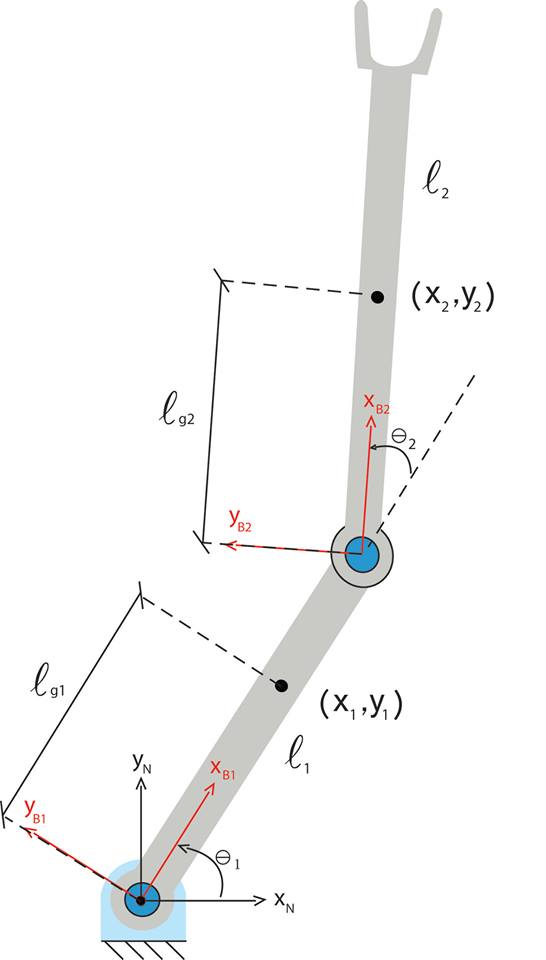
\includegraphics[scale=0.3]{RR.jpg}  
	\caption{Mecanismo \underline{R}\underline{R}}
	\label{fig:RR}
\end{figure}

\begin{itemize}
\item[1)] Defini\c{c}\~ao das coordenadas generalizadas:

\begin{equation}
\mq\ssh = \begin{bmatrix}
\theta_1 & \theta_2
\end{bmatrix}
\end{equation}

\begin{equation}
\mq\cir = \begin{bmatrix}
x_1 & y_1 & x_2 & y_2
\end{bmatrix}
\end{equation}

\item[2)] Defini\c{c}\~ao das velocidades generalizadas:

\begin{equation}
\mp\ssh = \begin{bmatrix}
\dot{\theta}_1 & \dot{\theta}_2
\end{bmatrix}
\end{equation}

\begin{equation}
\mp\cir = \begin{bmatrix}
\omega_{z1} & \omega_{z2} & v_{x1} & v_{y1} & v_{x2} & v_{y2}
\end{bmatrix}
\end{equation}

\item[3)] Cinem\'atica de posi\c{c}\~ao dos centros de massa e do efetuador utilizando matrizes de transforma\c{c}\~ao homog\^enea:

\begin{equation}
\hvct{\ttg_1}_{\ttB_1}  =
\begin{bmatrix} 
l_{g1} & 0 & 0 & 1
\end{bmatrix}^\msT
\end{equation}

\begin{equation}
\hvct{\ttg_2}_{\ttB_2}  =
\begin{bmatrix} 
l_{g2} & 0 & 0 & 1
\end{bmatrix}^\msT
\end{equation}

\begin{equation}
\hvct{\ttx}_{\ttB_2}  =
\begin{bmatrix} 
l_2 & 0 & 0 & 1
\end{bmatrix}^\msT
\end{equation}

\begin{equation}
\hvct{\mone}_{\ttN \rl \ttB_1} =
\begin{bmatrix}
\ccos_1 & -\ssin_1 & 0 & 0 \\
\ssin_1 & \ccos_1 & 0 & 0 \\
0 & 0 & 1 & 0 \\
0 & 0 & 0 & 1
\end{bmatrix}
\end{equation}

\begin{equation}
\hvct{\mone}_{\ttB_1 \rl \ttB_2} =
\begin{bmatrix}
\ccos_2 & -\ssin_2 & 0 & l_1 \\
\ssin_2 & \ccos_2 & 0 &  0 \\
0 & 0 & 1 & 0\\
0 & 0 & 0 & 1
\end{bmatrix}
\end{equation}

\begin{equation}
\hvct{\mone}_{\ttN \rl \ttB_2} = \hvct{\mone}_{\ttN \rl \ttB_1} \hvct{\mone}_{\ttB_1 \rl \ttB_2} =
\begin{bmatrix}
\ccos_{1\plus 2} & -\ssin_{1\plus 2} & 0 & l_1 \ccos_1\\
\ssin_{1\plus 2} & \ccos_{1\plus 2} & 0 & l_1 \ssin_1 \\
0 & 0 & 1 & 0\\
0 & 0 & 0 & 1
\end{bmatrix}
\end{equation}

\begin{equation}
\hvct{\ttg_1}_{\ttN}  = \hvct{\mone}_{\ttN \rl \ttB_1} \hvct{\ttg_1}_{\ttB_1} =
\begin{bmatrix}
l_{g1} \ccos_1 \\
l_{g1} \ssin_1 \\
0 \\
1
\end{bmatrix}
\end{equation}

\begin{equation}
\hvct{\ttg_2}_{\ttN}  = \hvct{\mone}_{\ttN \rl \ttB_2} \hvct{\ttg_2}_{\ttB_2} =
\begin{bmatrix}
l_1 \ccos_1 + l_{g2} \ccos_{1\plus 2} \\
l_1 \ssin_1 + l_{g2} \ssin_{1\plus 2} \\
0 \\
1
\end{bmatrix}
\end{equation}

\begin{equation}
\hvct{\ttx}_{\ttN}  = \hvct{\mone}_{\ttN \rl \ttB_2} \hvct{\ttx}_{\ttB_2} =
\begin{bmatrix}
l_1 \ccos_1 + l_2 \ccos_{1\plus 2} \\
l_1 \ssin_1 + l_2 \ssin_{1\plus 2} \\
0 \\
1
\end{bmatrix}
\end{equation}

\item[4)] Cinem\'atica de velocidades dos centros de massa:

\begin{equation}
[\underline{\vv}_1]_{\ttN} = \frac{\dd}{\dd t} [\ttg_1]_\ttN =
\begin{bmatrix}
-l_{g1} \ssin_1 \dot{\theta}_1 \\
 l_{g1} \ccos_1 \dot{\theta}_1 \\
 0 \\
\end{bmatrix}
\end{equation}

\begin{equation}
[\underline{\vv}_2]_{\ttN} = \frac{\dd}{\dd t} [\ttg_2]_\ttN =
\begin{bmatrix}
-l_{1} \ssin_1 \dot{\theta}_1 - l_{g2} \ssin_{1\plus 2} ( \dot{\theta}_1 + \dot{\theta}_2 )\\
 l_{1} \ccos_1 \dot{\theta}_1 + l_{g2} \ccos_{1\plus 2} ( \dot{\theta}_1 + \dot{\theta}_2 )\\
 0 \\
\end{bmatrix}
\end{equation}

\item[5)] Cinem\'atica de velocidades angulares das barras:

\begin{equation}
\smat{\underline{\vomega}_1}_{\ttB_1 \rl \ttB_1} = \tvct{\mone}_{\ttN \rl \ttB_1} \frac{\dd}{\dd t} \vct{\mone}_{\ttN \rl \ttB_1} = 
\begin{bmatrix}
0 & -\dot{\theta}_1 & 0 \\
\dot{\theta}_1 & 0 & 0 \\
0 & 0 & 0
\end{bmatrix}
\Rightarrow
\vct{\underline{\vomega}_1}_{\ttB_1} = 
\begin{bmatrix}
0 \\
0 \\
\dot{\theta}_1
\end{bmatrix}
\end{equation}

\begin{equation}
\smat{\underline{\vomega}_2}_{\ttB_2 \rl \ttB_2} = \tvct{\mone}_{\ttN \rl \ttB_2} \frac{\dd}{\dd t} \vct{\mone}_{\ttN \rl \ttB_2} = 
\begin{bmatrix}
0 & -\dot{\theta}_1 -\dot{\theta}_2 & 0 \\
\dot{\theta}_1 + \dot{\theta}_2 & 0 & 0 \\
0 & 0 & 0
\end{bmatrix}
\Rightarrow
\vct{\underline{\vomega}_2}_{\ttB_2} = 
\begin{bmatrix}
0 \\
0 \\
\dot{\theta}_1 + \dot{\theta}_2
\end{bmatrix}
\end{equation}

\item[6)] Montar o vetor $\underline{\mp}\cir(\mq\ssh,\mp\ssh)$ e calcular $\mC$, $\mA$ e $\mb$ atrav\'es das equa\c{c}\~oes \eqref{eq:MatrizC}, \eqref{eq:MatrizA} e \eqref{eq:Matrizb}:

\begin{equation}
\underline{\mp}\cir(\mq\ssh,\mp\ssh) =
\begin{bmatrix}
\dot{\theta}_1 \\
\dot{\theta}_1 + \dot{\theta}_2 \\
-l_{g1} \ssin_1 \dot{\theta}_1 \\
 l_{g1} \ccos_1 \dot{\theta}_1 \\
 -l_{1} \ssin_1 \dot{\theta}_1 - l_{g2} \ssin_{1\plus 2} ( \dot{\theta}_1 + \dot{\theta}_2 )\\
 l_{1} \ccos_1 \dot{\theta}_1 + l_{g2} \ccos_{1\plus 2} ( \dot{\theta}_1 + \dot{\theta}_2 )\\
\end{bmatrix}
\end{equation}

\begin{equation}
\frac{\partial \underline{\mp}\cir}{\partial \mp\ssh} =
\begin{bmatrix}
1 & 0 \\
1 & 1 \\
-l_{g1} \ssin_1 & 0 \\
 l_{g1} \ccos_1 & 0 \\
-l_{1} \ssin_1  - l_{g2} \ssin_{1\plus 2} & - l_{g2} \ssin_{1\plus 2} \\
 l_{1} \ssin_1  + l_{g2} \ccos_{1\plus 2} &   l_{g2} \ccos_{1\plus 2} \\
\end{bmatrix}
\end{equation}

\begin{equation}
\mC =
\begin{bmatrix}
1 & 0 \\
0 & 1 \\
1 & 0 \\
1 & 1 \\
-l_{g1} \ssin_1 & 0 \\
 l_{g1} \ccos_1 & 0 \\
-l_{1} \ssin_1  - l_{g2} \ssin_{1\plus 2} & - l_{g2} \ssin_{1\plus 2} \\
 l_{1} \ssin_1  + l_{g2} \ccos_{1\plus 2} &   l_{g2} \ccos_{1\plus 2} \\
\end{bmatrix}
\end{equation}

\begin{equation}
\mA =
\begin{bmatrix}
1 & 0 & -1 & 0 & 0 & 0 & 0 & 0 \\
1 & 1 & 0 & -1 & 0 & 0 & 0 & 0 \\
-l_{g1} \ssin_1 & 0 & 0 & 0 & -1 & 0 & 0 & 0 \\
 l_{g1} \ccos_1 & 0 & 0 & 0 & 0 & -1 & 0 & 0 \\
-l_{1} \ssin_1  - l_{g2} \ssin_{1\plus 2} & - l_{g2} \ssin_{1\plus 2} & 0 & 0 & 0 & 0 & -1 & 0 \\
 l_{1} \ccos_1  + l_{g2} \ccos_{1\plus 2} &   l_{g2} \ccos_{1\plus 2} & 0 & 0 & 0 & 0 & 0 & -1 \\
\end{bmatrix}
\end{equation}

\begin{equation}
\mb =
\begin{bmatrix}
0 \\
0 \\
l_{g1} \ccos_1 \dot{\theta}_1^2 \\
l_{g1} \ssin_1 \dot{\theta}_1^2 \\
l_{1} \ccos_1 \dot{\theta}_1^2  + l_{g2} \ccos_{1\plus 2}  (\dot{\theta}_1+\dot{\theta}_2)^2 \\
l_{1} \ssin_1  \dot{\theta}_1^2 + l_{g2} \ssin_{1\plus 2}   (\dot{\theta}_1+\dot{\theta}_2)^2 \\
\end{bmatrix}
\end{equation}

\item[7)] Calcular a energia de acelera\c{c}\~oes $S$:

\begin{equation}
S = \frac{1}{2} \Big( m_1 (\dot{v}_{x1}^2 + \dot{v}_{y1}^2) + m_2 (\dot{v}_{x2}^2 + \dot{v}_{y2}^2) + J_{z1} \dot{\omega}_{z1}^2 + + J_{z2} \dot{\omega}_{z2}^2 \Big)
\end{equation}

\item[8)] Obter $\mM$ e $\mv$ utilizando as equa\c{c}\~oes \eqref{eq:MatrizM} e \eqref{eq:Matrizv}:

\begin{equation}
\mM = \begin{bmatrix}
0 & 0 & J_{z1} & J_{z2} & m_1 & m_1 & m_2 & m_2
\end{bmatrix}^\msD
\end{equation}

\begin{equation}
\mv = \mzr
\end{equation}

\item[9)] Montar os vetores $\mf$, $\mg$ e $\mu$:

\begin{equation}
\mf =
\begin{bmatrix}
c_1 \dot{\theta}_1 + \gamma_1 \sign (\dot{\theta}_1) \\
c_2 \dot{\theta}_2 + \gamma_2 \sign (\dot{\theta}_2) \\
0 \\
0 \\
0 \\
0 \\
0 \\
0 \\
\end{bmatrix}
\end{equation}

\begin{equation}
\mg =
\begin{bmatrix}
0 \\
0 \\
0 \\
0 \\
0 \\
m_1 g \\
0 \\
m_2 g
\end{bmatrix}
\end{equation}

\begin{equation}
\mu =
\begin{bmatrix}
\tau_1 \\
\tau_2
\end{bmatrix}
\end{equation}

\end{itemize}

Sendo assim, a partir da equa\c{c}\~ao \eqref{eq:DinamicaDireta}, temos que o modelo para simula\c{c}\~ao din\^amica direta do mecanismo \underline{R}\underline{R} \'e dado por:

\small\begin{equation} \label{eq:RR}
\begin{cases}
\begin{bmatrix}
1 & 0 \\
0 & 1 \\
1 & 0 \\
1 & 1 \\
-l_{g1} \ssin_1 & 0 \\
 l_{g1} \ccos_1 & 0 \\
-l_{1} \ssin_1  - l_{g2} \ssin_{1\plus 2} & - l_{g2} \ssin_{1\plus 2} \\
 l_{1} \ssin_1  + l_{g2} \ccos_{1\plus 2} &   l_{g2} \ccos_{1\plus 2} \\
\end{bmatrix}^\msT
\begin{Bmatrix}
\begin{bmatrix}
0 \\ 0 \\ J_{z1} \\ J_{z2} \\ m_1 \\ m_1 \\ m_2 \\ m_2
\end{bmatrix}^\msD
\begin{bmatrix}
\ddot{\theta}_1 \\
\ddot{\theta}_2 \\
\dot{\omega}_{z1} \\
\dot{\omega}_{z2} \\
\dot{v}_{x1} \\
\dot{v}_{y1} \\
\dot{v}_{x2} \\
\dot{v}_{y2} \\
\end{bmatrix}
+
\begin{bmatrix}
c_1 \dot{\theta}_1 + \gamma_1 \sign (\dot{\theta}_1) \\
c_2 \dot{\theta}_2 + \gamma_2 \sign (\dot{\theta}_2) \\
0 \\
0 \\
0 \\
0 \\
0 \\
0 \\
\end{bmatrix}
+
\begin{bmatrix}
0 \\
0 \\
0 \\
0 \\
0 \\
m_1 g \\
0 \\
m_2 g
\end{bmatrix}
\end{Bmatrix}
=
\begin{bmatrix}
\tau_1 \\ \tau_2
\end{bmatrix} \\
\begin{bmatrix}
1 & 0 & -1 & 0 & 0 & 0 & 0 & 0 \\
1 & 1 & 0 & -1 & 0 & 0 & 0 & 0 \\
-l_{g1} \ssin_1 & 0 & 0 & 0 & -1 & 0 & 0 & 0 \\
 l_{g1} \ccos_1 & 0 & 0 & 0 & 0 & -1 & 0 & 0 \\
-l_{1} \ssin_1  - l_{g2} \ssin_{1\plus 2} & - l_{g2} \ssin_{1\plus 2} & 0 & 0 & 0 & 0 & -1 & 0 \\
 l_{1} \ccos_1  + l_{g2} \ccos_{1\plus 2} &   l_{g2} \ccos_{1\plus 2} & 0 & 0 & 0 & 0 & 0 & -1 \\
\end{bmatrix}
\begin{bmatrix}
\ddot{\theta}_1 \\
\ddot{\theta}_2 \\
\dot{\omega}_{z1} \\
\dot{\omega}_{z2} \\
\dot{v}_{x1} \\
\dot{v}_{y1} \\
\dot{v}_{x2} \\
\dot{v}_{y2} \\
\end{bmatrix} = 
\begin{bmatrix}
0 \\
0 \\
l_{g1} \ccos_1 \dot{\theta}_1^2 \\
l_{g1} \ssin_1 \dot{\theta}_1^2 \\
l_{1} \ccos_1 \dot{\theta}_1^2  + l_{g2} \ccos_{1\plus 2}  (\dot{\theta}_1+\dot{\theta}_2)^2 \\
l_{1} \ssin_1  \dot{\theta}_1^2 + l_{g2} \ssin_{1\plus 2}   (\dot{\theta}_1+\dot{\theta}_2)^2 \\
\end{bmatrix}
\end{cases}
\end{equation}\normalsize

Para realizar a modelagem de mecanismos paralelos a partir de subsistemas seriais j\'a deduzidos, \'e necess\'ario introduzir mais alguns conceitos: \\

Sejam $\ssB_0$, $\ssB_1$, ..., $\ssB_{n-1}$ $n$ subsistemas mec\^anicos e $\ssM$ um sistema mec\^anico de $\nu\ssh$ graus de liberdade gerado pelo acoplamento dos subsistemas citados. Definimos:

\begin{itemize}
\item $\mq_0$: vetor de coordenadas generalizas da plataforma/efetuador de $\ssM$.
\item $\mq_j\ssh, \,j=1, ..., n-1$: vetor de coordenadas generalizadas independentes do subsistema  $\ssB_j$.
\item $\mq\hcir$: vetor de coordenadas generalizadas redundantes n\~ao pertencentes \`a plataforma/efetuador. Definido como $\mq\hcir = \begin{bmatrix}  {\mq_1\ssh}^\msT & ... & {\mq_{n-1}\ssh}^\msT \end{bmatrix}^\msT $.
\item $\mq$: vetor contendo todas as coordenadas generalizadas do sistema $\ssM$. Definido como $\mq = \begin{bmatrix} \mq_0^\msT & {\mq\hcir}^\msT \end{bmatrix}^\msT $.
\item $\overline{\mq}(\mq)$: vetor dos v\'inculos de posi\c{c}\~ao entre subsistemas. As equa\c{c}\~oes v\'inculares s\~ao dadas por $\overline{\mq}(\mq) = \mzr $.
\item $\mp\ssh_0$: vetor de velocidades generalizadas independentes da plataforma/efetuador de $\ssM$. É definido por $\mp\ssh_0 = \mD(\mq_0)\dot{\mq}_0$, sendo $\mD(\mq_0)$ tal que $\dot{\mq}_0  = \mD^+(\mq_0) \mp\ssh_0$.
\item $\mp_j\ssh, \,j=1, ..., n-1$: vetor de velocidades generalizadas independentes do subsistema  $\ssB_j$. É definido por $\mp_j\ssh = \dot{\mq}_j\ssh$.
\item $\mp_j\cir, \,j=1, ..., n-1$: vetor de velocidades generalizadas redundantes do subsistema  $\ssB_j$.
\item $\mp_j, \,j=1, ..., n-1$: vetor de velocidades generalizadas do subsistema  $\ssB_j$. É definido por $\mp_j = \begin{bmatrix} {\mp_j\ssh}^\msT & {\mp_j\cir}^\msT \end{bmatrix}$.
\item $\mp\ssh$: vetor de $\nu\ssh$ velocidades generalizadas independentes de $\ssM$. É dado por $\mp\ssh = \mp_0\ssh$.
\item $\mp\cir$: vetor de $\nu\ssh$ velocidades generalizadas redundantes de $\ssM$. É definido por $\mp\cir = \begin{bmatrix} \mp_1^\msT & \mp_2^\msT & ... & \mp_{n-1}^\msT \end{bmatrix}^\msT $.
\item $\mp$: vetor contendo todas as velocidades generalizadas de $\ssM$. É definido por $\mp = \begin{bmatrix} {\mp\ssh}^\msT & {\mp\cir}^\msT \end{bmatrix}^\msT $.
\item $\mrho$: vetor definido como $\mrho = \begin{bmatrix} {\mrho\ssh}^\msT & {\mrho\cir}^\msT \end{bmatrix}^\msT $, sendo $\mrho\ssh = \mp_0\ssh$ e $\mrho\cir = \dot{\mq}\hcir $.
\item $\overline{\mrho}(\mrho)$: vetor dos v\'inculos de velocidades entre subsistemas. As equa\c{c}\~oes v\'inculares s\~ao dadas por $\overline{\mrho}(\mrho) = \mzr $.
\item $\mA_j(\mq_j\ssh), \,j=0, ..., n-1$: Jacobiano dos v\'inculos de velocidades do subsistema $\ssB_j$.
\item $\mC_j(\mq_j\ssh), \,j=0, ..., n-1$: complemento ortogonal do Jacobiano dos v\'inculos de velocidades do subsistema $\ssB_j$.
\item $\mM_j, \,j=0, ..., n-1$: matriz de in\'ercia desacoplada do subsistema $\ssB_j$.
\item $\mv_j(\mp_j\ssh), \,j=0, ..., n-1 $: vetor dos termos girosc\'opicos desacoplados do subsistema $\ssB_j$.
\item $\mf_j(\mq_j\ssh), \,j=0, ..., n-1$: vetor dos esfor\c{c}os de atrito do subsistema $\ssB_j$.
\item $\mg_j, \,j=0, ..., n-1$: vetor dos esfor\c{c}os gravitacionais do subsistema $\ssB_j$.
\item $\mu_j, \,j=0, ..., n-1$: vetor dos esfor\c{c}os ativos externos do subsistema $\ssB_j$.
\end{itemize}

O modelo para simula\c{c}\~ao din\^amica direta \'e dado pelo seguinte equacionamento:

\begin{equation} \label{eq:DinamicaDireta2}
\begin{cases}
\dot{\mq}_0 = \mD^+ (\mq_0) \mp\ssh \\
\mC^\msT(\mq) \Big( \mM \dot{\mp} + \mv(\mp) + \mf(\mp) + \mg \Big) = \hat{\mC}^\msT(\mq) \mu \\
\mA(\mq) \dot{\mp} = \mb(\mq,\mp)
\end{cases}
\end{equation}

Sendo:

\begin{equation} \label{eq:VinculosVelocidades}
\overline{\mrho} = \frac{\partial \overline{\mq}}{\partial \mq_0} \mD^+ \mrho\ssh + \frac{\partial \overline{\mq}}{\partial \mq\hcir}  \mrho\cir
\end{equation}

\begin{equation} \label{eq:MatrizCchapeu}
\hat{\mC} = \begin{bmatrix}
\mone \\
- \displaystyle\frac{\partial \overline{\mq}}{\partial \mq\hcir}^\msI  \frac{\partial \overline{\mq}}{\partial \mq_0 }\cdot\mD^+
\end{bmatrix}
\end{equation}

\begin{equation} \label{eq:MatrizC2}
\mC = 
\begin{bmatrix}
\mC_0 &  \mzr  & \ldots & \mzr\\
\mzr  &  \mC_1 & \ldots & \mzr\\
\vdots & \vdots & \ddots & \vdots\\
\mzr  &   \mzr       &\ldots & \mC_{n-1}
\end{bmatrix}
\hat{\mC}
\end{equation}

\begin{equation} \label{eq:MatrizA2}
\mA = 
\begin{bmatrix}
\begin{bmatrix}
\mzr &  \mA_1  & \mzr & \ldots & \mzr\\
\mzr  &  \mzr & \mA_2 & \ldots & \mzr\\
\vdots & \vdots & \vdots & \ddots & \vdots\\
\mzr  &   \mzr  & \mzr     &\ldots & \mA_{n-1}
\end{bmatrix} \\
\displaystyle\frac{\partial \overline{\mrho}}{\partial \mp}
\end{bmatrix}
\end{equation}

\begin{equation} \label{eq:Matrizb2}
\mb = - \dot{\mA}(\mq,\mp) \mp
\end{equation}

\begin{equation} \label{eq:MatrizM2}
\mM =
\begin{bmatrix}
\mM_0 &  \mzr  & \ldots & \mzr\\
\mzr  &  \mM_1 & \ldots & \mzr\\
\vdots & \vdots & \ddots & \vdots\\
\mzr  &   \mzr       &\ldots & \mM_{n-1}
\end{bmatrix}
\end{equation}

\begin{equation} \label{eq:Matrizv2}
\mv = \begin{bmatrix}
\mv_0^\msT & \mv_1^\msT & ... & \mv_{n-1}^\msT
\end{bmatrix}^\msT
\end{equation}

\begin{equation} \label{eq:Matrizf2}
\mf = \begin{bmatrix}
\mf_0^\msT & \mf_1^\msT & ... & \mf_{n-1}^\msT
\end{bmatrix}^\msT
\end{equation}

\begin{equation} \label{eq:Matrizg2}
\mg = \begin{bmatrix}
\mg_0^\msT & \mg_1^\msT & ... & \mg_{n-1}^\msT
\end{bmatrix}^\msT
\end{equation}

\begin{equation}
\mu =
\begin{bmatrix} \label{eq:Matrizu}
\mu_0^\msT & \mu_1^\msT & ... & \mu_{n-1}^\msT
\end{bmatrix}^\msT
\end{equation}

Aqui seguem as etapas do algoritmo para dedu\c{c}\~ao do modelo din\^amico de um subsistema serial acompanhado de um exemplo de aplica\c{c}\~ao para dedu\c{c}\~ao do modelo din\^amico do mecanismo 5R (pent\'agono articulado) a partir do acoplamento dos modelos de 2 mecanismos \underline{R}\underline{R} e uma massa pontual (efetuador).

\begin{figure}[H]
	\centering
	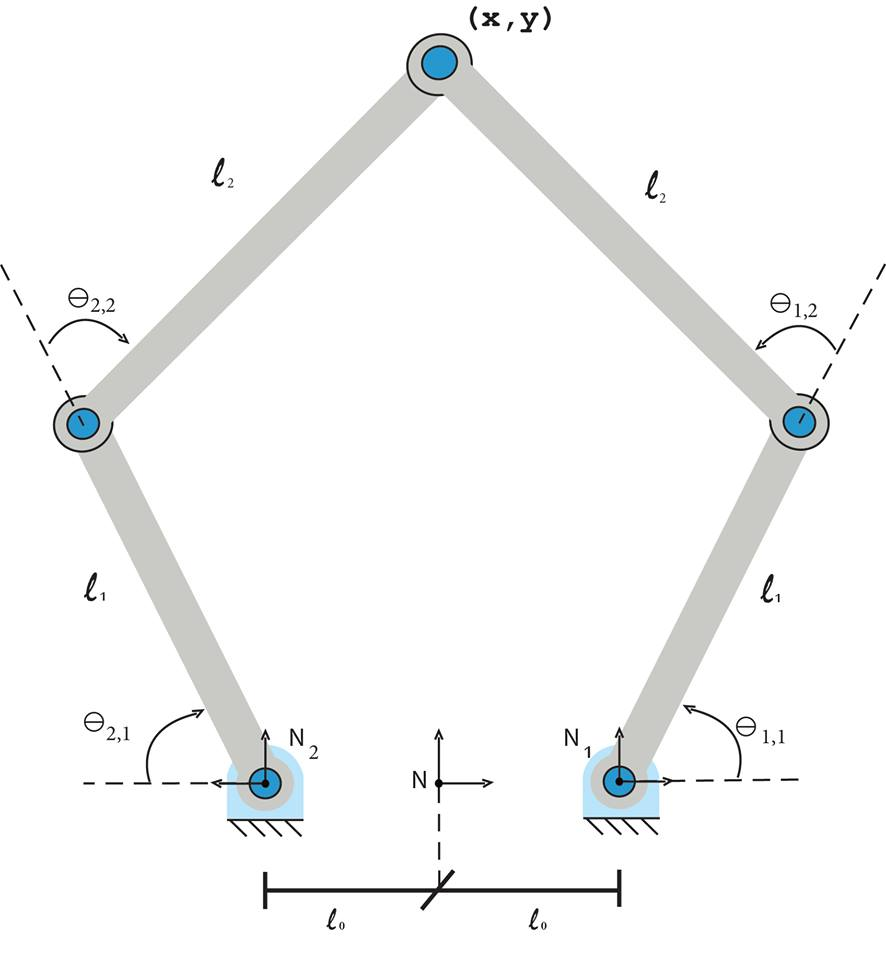
\includegraphics[scale=0.4]{5Rscan.jpg}
	\caption{Mecanismo 5R}
	\label{fig:RR}
\end{figure}

O modelo do mecanismo \underline{R}\underline{R} \'e dado pela equa\c{c}\~ao \eqref{eq:RR}. O modelo da massa pontual \'e dado pela seguinte express\~ao:

\begin{equation} \label{eq:MassaPontual}
\begin{cases}
\begin{bmatrix}
\dot{x} \\
\dot{y}
\end{bmatrix}
=
\begin{bmatrix}
1 & 0 \\
0 & 1
\end{bmatrix}
\begin{bmatrix}
v_{x} \\
v_{y}
\end{bmatrix}
\\
\begin{bmatrix}
m_0 \\
m_0 \\
\end{bmatrix}^\msD
\begin{bmatrix}
\dot{v}_{x} \\
\dot{v}_{y}
\end{bmatrix}
+
\begin{bmatrix}
0 \\
m_0 g
\end{bmatrix}
=
\begin{bmatrix}
0 \\
0
\end{bmatrix}
\end{cases}
\end{equation}

Etapas do algoritmo:

\begin{itemize}
\item[1)] Defini\c{c}\~ao das coordenadas generalizadas:

\begin{equation}
\mq_0 = \begin{bmatrix}
x & y
\end{bmatrix}^\msT
\end{equation}
\begin{equation}
\mq_1\ssh = \begin{bmatrix}
\theta_{1,1} &
\theta_{1,2} 
\end{bmatrix}^\msT
\end{equation}
\begin{equation}
\mq_2\ssh = \begin{bmatrix}
\theta_{2,1} &
\theta_{2,2}
\end{bmatrix}^\msT
\end{equation}

\item[2)] Defini\c{c}\~ao das velocidades generalizadas:

\begin{equation}
\mp_0\ssh = \begin{bmatrix}
\dot{x} & \dot{y} \\
\end{bmatrix}^\msT
\Rightarrow \mD = \mone
\end{equation}
\begin{equation}
\mp_1\cir = \begin{bmatrix}
\omega_{1,z1} & \omega_{1,z2} & v_{1,x1} & v_{1,y1} & v_{1,x2} & v_{1,y2}
\end{bmatrix}^\msT
\end{equation}
\begin{equation}
\mp_2\cir = \begin{bmatrix}
\omega_{2,z1} & \omega_{2,z2} & v_{2,x1} & v_{2,y1} & v_{2,x2} & v_{2,y2}
\end{bmatrix}^\msT
\end{equation}

\item[3)] Defini\c{c}\~ao dos v\'inculos de posi\c{c}\~ao utilizando matrizes de transforma\c{c}\~ao homog\^enea:

\begin{equation}
\hvct{\mone}_{\ttN \rl \ttN_1} =
\begin{bmatrix}
1 & 0 & 0 & l_0 \\
0 & 1 & 0 & 0 \\
0 & 0 & 1 & 0 \\
0 & 0 & 0 & 1
\end{bmatrix}
\end{equation}

\begin{equation}
\hvct{\mone}_{\ttN \rl \ttN_2} =
\begin{bmatrix}
-1 & 0 & 0 & -l_0 \\
0 & 1 & 0 & 0 \\
0 & 0 & -1 & 0\\
0 & 0 & 0 & 1
\end{bmatrix}
\end{equation}

\begin{equation}
\vct{\ttx_0}_{\ttN} =
\begin{bmatrix}
x \\
y \\
0 \\
\end{bmatrix}
\end{equation}

\begin{equation}
\vct{\ttx_1}_{\ttN_1} =
\begin{bmatrix}
l_1 \ccos_{1,1} + l_2 \ccos_{1,1\plus 2} \\
l_1 \ssin_{1,1} + l_2 \ssin_{1,1\plus 2} \\
0
\end{bmatrix}
\end{equation}

\begin{equation}
\vct{\ttx_2}_{\ttN_2} =
\begin{bmatrix}
l_1 \ccos_{2,1} + l_2 \ccos_{2,1\plus 2} \\
l_1 \ssin_{2,1} + l_2 \ssin_{2,1\plus 2} \\
0
\end{bmatrix}
\end{equation}

\begin{equation}
\hvct{\ttx_1}_{\ttN} = \hvct{\mone}_{\ttN \rl \ttN_1} \hvct{\ttx_1}_{\ttN_1} =
\begin{bmatrix}
l_0 + l_1 \ccos_{1,1} + l_2 \ccos_{1,1\plus 2} \\
l_1 \ssin_{1,1} + l_2 \ssin_{1,1\plus 2} \\
0 \\
1
\end{bmatrix}
\end{equation}

\begin{equation}
\hvct{\ttx_2}_{\ttN} = \hvct{\mone}_{\ttN \rl \ttN_2} \hvct{\ttx_2}_{\ttN_2} =
\begin{bmatrix}
-l_0 - l_1 \ccos_{2,1} - l_2 \ccos_{2,1\plus 2} \\
l_1 \ssin_{2,1} + l_2 \ssin_{2,1\plus 2} \\
0 \\
1
\end{bmatrix}
\end{equation}

V\'inculos de posi\c{c}\~ao:

\begin{equation}
\begin{cases}
\vct{\ttx_0}_{\ttN} = \vct{\ttx_1}_{\ttN} \\
\vct{\ttx_0}_{\ttN} = \vct{\ttx_2}_{\ttN} \\
\end{cases}
\Rightarrow
\begin{cases}
x = l_0 + l_1 \ccos_{1,1} + l_2 \ccos_{1,1\plus 2} \\
y = l_1 \ssin_{1,1} + l_2 \ssin_{1,1\plus 2} \\ 
x = -l_0 - l_1 \ccos_{2,1} - l_2 \ccos_{2,1\plus 2} \\
y = l_1 \ssin_{2,1} + l_2 \ssin_{2,1\plus 2} \\
\end{cases}
\end{equation}

\begin{equation}
\therefore \overline{\mq}(\mq) = 
\begin{bmatrix}
x - l_0 - l_1 \ccos_{1,1} - l_2 \ccos_{1,1\plus 2} \\
y - l_1 \ssin_{1,1} - l_2 \ssin_{1,1\plus 2} \\
x + l_0 + l_1 \ccos_{2,1} + l_2 \ccos_{2,1\plus 2} \\
y - l_1 \ssin_{2,1} - l_2 \ssin_{2,1\plus 2} \\
\end{bmatrix}
= \mzr
\end{equation}

\item[4)] C\'alculo dos Jacobianos dos v\'inculos de posi\c{c}\~ao e defini\c{c}\~ao dos v\'inculos de velocidades:

\begin{equation}
\frac{\partial \overline{\mq}}{\partial \mq_0} = 
\begin{bmatrix}
1 & 0 \\
0 & 1 \\
1 & 0 \\
0 & 1 \\
\end{bmatrix}
\end{equation}

\begin{equation}
\frac{\partial \overline{\mq}}{\partial \mq\hcir} = 
\begin{bmatrix}
 l_1 \ssin_{1,1} + l_2 \ssin_{1\plus 2} &  l_2 \ssin_{1\plus 2} & 0 & 0 \\
-l_1 \ccos_{1,1} - l_2 \ccos_{1\plus 2} & -l_2 \ccos_{1\plus 2} & 0 & 0  \\
0 & 0 & -l_1 \ssin_{2,1} - l_2 \ssin_{2\plus 2} & -l_2 \ssin_{2\plus 2}  \\
0 & 0 & -l_1 \ccos_{2,1} - l_2 \ccos_{2\plus 2} & -l_2 \ccos_{2\plus 2}   \\
\end{bmatrix}
\end{equation}

\begin{equation}
\overline{\mrho} =  
\begin{bmatrix}
1 & 0 \\
0 & 1 \\
1 & 0 \\
0 & 1 \\
\end{bmatrix}
\begin{bmatrix}
\dot{x} \\
\dot{y} \\
\end{bmatrix}
+ 
 \begin{bmatrix}
 l_1 \ssin_{1,1} + l_2 \ssin_{1\plus 2} &  l_2 \ssin_{1\plus 2} & 0 & 0 \\
-l_1 \ccos_{1,1} - l_2 \ccos_{1\plus 2} & -l_2 \ccos_{1\plus 2} & 0 & 0  \\
0 & 0 & -l_1 \ssin_{2,1} - l_2 \ssin_{2\plus 2} & -l_2 \ssin_{2\plus 2}  \\
0 & 0 & -l_1 \ccos_{2,1} - l_2 \ccos_{2\plus 2} & -l_2 \ccos_{2\plus 2}   \\
\end{bmatrix}
\begin{bmatrix}
\dot{\theta}_{1,1} \\
\dot{\theta}_{1,2} \\
\dot{\theta}_{2,1} \\
\dot{\theta}_{2,2} \\
\end{bmatrix} = \mzr
\end{equation}

\item[5)] C\'alculo de $\hat{\mC}$, $\mC$, $\mA$ e $\mb$ atrav\'es de \eqref{eq:MatrizCchapeu}, \eqref{eq:MatrizC2}, \eqref{eq:MatrizA2} e \eqref{eq:Matrizb2}:

\begin{equation}
\hat{\mC} =
\begin{bmatrix}
1 & 0 \\
0 & 1 \\
\displaystyle\frac{\ccos_{1,1\plus 2}}{l_1 \ssin_{1,2}} & \displaystyle\frac{\ssin_{1,1\plus 2}}{l_1 \ssin_{1,2}} \\
-\displaystyle\frac{l_1\ccos_{1,1} + l_2\ccos_{1,1\plus 2}}{l_1 l_2 \ssin_{1,2}} & -\displaystyle\frac{l_1\ssin_{1,1} + l_2\ssin_{1,1\plus 2}}{l_1 l_2 \ssin_{1,2}} \\
-\displaystyle\frac{\ccos_{2,1\plus 2}}{l_1 \ssin_{2,2}} & \displaystyle\frac{\ssin_{2,1\plus 2}}{l_1 \ssin_{2,2}} \\
\displaystyle\frac{l_1\ccos_{2,1} + l_2\ccos_{2,1\plus 2}}{l_1 l_2 \ssin_{2,2}} & -\displaystyle\frac{l_1\ssin_{2,1} + l_2\ssin_{2,1\plus 2}}{l_1 l_2 \ssin_{2,2}} \\
\end{bmatrix}
\end{equation}

\footnotesize\begin{equation}
\mC =
\begin{bmatrix}
1 & 0 \\
0 & 1 \\
\displaystyle\frac{\ccos_{1,1\plus 2}}{l_1 s_{1,2}} & \displaystyle\frac{\ssin_{1,1\plus 2}}{l_1 s_{1,2}} \\
-\displaystyle\frac{l_1 \ccos_{1,1} + l_2 \ccos_{1,1\plus 2}}{l_1 l_2 \ssin_{1,2}} & -\displaystyle\frac{l_1 \ssin_{1,1} + l_2 \ssin_{1,1\plus 2}}{l_1 l_2 \ssin_{1,2}} \\
\displaystyle\frac{\ccos_{1,1\plus 2}}{l_1 s_{1,2}} & \displaystyle\frac{\ssin_{1,1\plus 2}}{l_1 s_{1,2}} \\
-\displaystyle\frac{\ccos_{\theta_{1,1}}}{l_2 s_{1,2}} & -\displaystyle\frac{\ssin_{\theta_{1,1}}}{l_2 s_{1,2}} \\
-\displaystyle\frac{l_{g1} \ssin_{1,1} \ccos_{1,1\plus 2}}{l_1 \ssin_{1,2}} & -\displaystyle\frac{l_{g1} \ssin_{1,1} \ssin_{1,1\plus 2}}{l_1 \ssin_{1,2}} \\
\displaystyle\frac{l_{g1} \ccos_{1,1} \ccos_{1,1\plus 2}}{l_1 \ssin_{1,2}} & \displaystyle\frac{l_{g1} \ccos_{1,1} \ssin_{1,1\plus 2}}{l_1 \ssin_{1,2}} \\
-\displaystyle\frac{l_2 \ssin_{1,1}\ccos_{1,1\plus 2} - l_{g2} \ccos_{1,1} \ssin_{1,1\plus 2} }{l_2 \ssin_{1,2}} & -\displaystyle\frac{(l_2 - l_{g2}) \ssin_{1,1}\ssin_{1,1\plus 2} }{l_2 \ssin_{1,2}} \\
\displaystyle\frac{(l_2 - l_{g2}) \ccos_{1,1}\ccos_{1,1\plus 2} }{l_2 \ssin_{1,2}} & -\displaystyle\frac{l_2 \ccos_{1,1}\ssin_{1,1\plus 2} - l_{g2} \ssin_{1,1} \ccos_{1,1\plus 2} }{l_2 \ssin_{1,2}} \\
-\displaystyle\frac{\ccos_{2,1\plus 2}}{l_1 s_{2,2}} & \displaystyle\frac{\ssin_{2,1\plus 2}}{l_1 s_{2,2}} \\
\displaystyle\frac{l_1 \ccos_{2,1} + l_2 \ccos_{2,1\plus 2}}{l_1 l_2 \ssin_{2,2}} & -\displaystyle\frac{l_1 \ssin_{2,1} + l_2 \ssin_{2,1\plus 2}}{l_1 l_2 \ssin_{2,2}} \\
-\displaystyle\frac{\ccos_{2,1\plus 2}}{l_1 s_{2,2}} & \displaystyle\frac{\ssin_{2,1\plus 2}}{l_1 s_{2,2}} \\
\displaystyle\frac{\ccos_{2,1}}{l_2 s_{2,2}} & -\displaystyle\frac{\ssin_{2,1}}{l_2 s_{2,2}} \\
\displaystyle\frac{l_{g1} \ssin_{2,1} \ccos_{2,1\plus 2}}{l_1 \ssin_{2,2}} & -\displaystyle\frac{l_{g1} \ssin_{2,1} \ssin_{2,1\plus 2}}{l_1 \ssin_{2,2}} \\
-\displaystyle\frac{l_{g1} \ccos_{2,1} \ccos_{2,1\plus 2}}{l_1 \ssin_{2,2}} & \displaystyle\frac{l_{g1} \ccos_{2,1} \ssin_{2,1\plus 2}}{l_1 \ssin_{2,2}} \\
\displaystyle\frac{l_2 \ssin_{2,1}\ccos_{2,1\plus 2} - l_{g2} \ccos_{2,1} \ssin_{2,1\plus 2} }{l_2 \ssin_{2,2}} & -\displaystyle\frac{(l_2 - l_{g2}) \ssin_{2,1}\ssin_{2,1\plus 2} }{l_2 \ssin_{2,2}} \\
\displaystyle\frac{(l_2 - l_{g2}) \ccos_{2,1}\ccos_{2,1\plus 2} }{l_2 \ssin_{2,2}} & -\displaystyle\frac{l_2 \ccos_{2,1}\ssin_{2,1\plus 2} - l_{g2} \ssin_{2,1} \ccos_{2,1\plus 2} }{l_2 \ssin_{2,2}} \\
\end{bmatrix}
\end{equation}\normalsize

\end{itemize}

\footnotesize\begin{equation}
\mA =\begin{bmatrix}
0 & 0 &1 & 0 & \mminus 1 & 0 & 0 & 0 & 0 & 0 & 0 & 0 & 0 & 0 & 0 & 0 & 0 & 0 \\
0 & 0 &1 & 1 & 0 & \mminus 1 & 0 & 0 & 0 & 0 & 0 & 0 & 0 & 0 & 0 & 0 & 0 & 0 \\
0 & 0 &\mminus l_{g1} \ssin_1 & 0 & 0 & 0 & \mminus 1 & 0 & 0 & 0 & 0 & 0 & 0 & 0 & 0 & 0 & 0 & 0 \\
0 & 0 & l_{g1} \ccos_1 & 0 & 0 & 0 & 0 & \mminus 1 & 0 & 0 & 0 & 0 & 0 & 0 & 0 & 0 & 0 & 0 \\
0 & 0 &\mminus l_{1} \ssin_1  \mminus  l_{g2} \ssin_{1\plus 2} & \mminus  l_{g2} \ssin_{1\plus 2} & 0 & 0 & 0 & 0 & \mminus 1 & 0  & 0 & 0 & 0 & 0 & 0 & 0 & 0 & 0 \\
0 & 0 & l_{1} \ccos_1  \pplus l_{g2} \ccos_{1\plus 2} &   l_{g2} \ccos_{1\plus 2} & 0 & 0 & 0 & 0 & 0 & \mminus 1 & 0 & 0 & 0 & 0 & 0 & 0 & 0 & 0 \\
0 & 0 & 0 & 0 & 0 & 0 & 0 & 0 & 0 & 0 & 1 & 0 & \mminus 1 & 0 & 0 & 0 & 0 & 0 \\
0 & 0 & 0 & 0 & 0 & 0 & 0 & 0 & 0 & 0 & 1 & 1 & 0 & \mminus 1 & 0 & 0 & 0 & 0 \\
0 & 0 & 0 & 0 & 0 & 0 & 0 & 0 & 0 & 0 & \mminus l_{g1} \ssin_1 & 0 & 0 & 0 & \mminus 1 & 0 & 0 & 0 \\
0 & 0 & 0 & 0 & 0 & 0 & 0 & 0 & 0 & 0 &  l_{g1} \ccos_1 & 0 & 0 & 0 & 0 & \mminus 1 & 0 & 0\\
0 & 0 & 0 & 0 & 0 & 0 & 0 & 0 & 0 & 0 & \mminus l_{1} \ssin_1  \mminus  l_{g2} \ssin_{1\plus 2} & \mminus  l_{g2} \ssin_{1\plus 2} & 0 & 0 & 0 & 0 & \mminus 1 & 0 \\
0 & 0 & 0 & 0 & 0 & 0 & 0 & 0 & 0 & 0 & l_{1} \ccos_1  \pplus l_{g2} \ccos_{1 \plus 2} &   l_{g2} \ccos_{1 \plus 2} & 0 & 0 & 0 & 0 & 0 & \mminus 1 \\
1 & 0 & l_1 \ssin_{1,1} \pplus l_2 \ssin_{1\plus 2} &  l_2 \ssin_{1\plus 2} & 0 & 0 & 0 & 0 & 0 & 0 & 0 & 0 & 0 & 0 & 0 & 0 & 0 & 0  \\
0 & 1 & \mminus l_1 \ccos_{1,1} \mminus l_2 \ccos_{1\plus 2} & \mminus l_2 \ccos_{1\plus 2} & 0 & 0 & 0 & 0 & 0 & 0 & 0 & 0 & 0 & 0 & 0 & 0 & 0 & 0  \\
1 & 0 & 0 & 0 & 0 & 0 & 0 & 0 & 0 & 0 & \mminus l_1 \ssin_{2,1} \mminus l_2 \ssin_{2\plus 2} & \mminus l_2 \ssin_{2\plus 2} & 0 & 0 & 0 & 0 & 0 & 0  \\
0 & 1 & 0 & 0 & 0 & 0 & 0 & 0 & 0 & 0 & \mminus l_1 \ccos_{2,1} \mminus  l_2 \ccos_{2\plus 2} & \mminus l_2 \ccos_{2\plus 2} & 0 & 0 & 0 & 0 & 0 & 0  \\
\end{bmatrix}
\end{equation}\normalsize

\begin{equation}
\mb =
\begin{bmatrix}
0 \\
0 \\
l_{g1} \ccos_{1,1} \dot{\theta}_{1,1}^2 \\
l_{g1} \ssin_{1,1} \dot{\theta}_{1,1}^2 \\
l_{1} \ccos_{1,1} \dot{\theta}_{1,1}^2  + l_{g2} \ccos_{1, 1\plus 2}  (\dot{\theta}_{1,1}+\dot{\theta}_{1,2})^2 \\
l_{1} \ssin_{1,1}  \dot{\theta}_{1,1}^2 + l_{g2} \ssin_{1, 1\plus 2}   (\dot{\theta}_{1,1}+\dot{\theta}_{1,2})^2 \\
0 \\
0 \\
l_{g1} \ccos_{2,1} \dot{\theta}_{2,1}^2 \\
l_{g1} \ssin_{2,1} \dot{\theta}_{2,1}^2 \\
l_{2} \ccos_{2,1} \dot{\theta}_{2,1}^2  + l_{g2} \ccos_{2, 1\plus 2}  (\dot{\theta}_{2,1}+\dot{\theta}_{2,2})^2 \\
l_{2} \ssin_{2,1}  \dot{\theta}_{2,1}^2 + l_{g2} \ssin_{2, 1\plus 2}   (\dot{\theta}_{2,1}+\dot{\theta}_{2,2})^2 \\
-l_1 \ccos_{1,1} \dot{\theta}_{1,1}^2 - l_2 \ccos_{1,1\plus 2} (\dot{\theta}_{1,1} + \dot{\theta}_{1,2})^2 \\
-l_1 \ssin_{1,1} \dot{\theta}_{1,1}^2 - l_2 \ssin_{1,1\plus 2} (\dot{\theta}_{1,1} + \dot{\theta}_{1,2})^2 \\
 l_1 \ccos_{2,1} \dot{\theta}_{2,1}^2 + l_2 \ccos_{2,1\plus 2} (\dot{\theta}_{2,1} + \dot{\theta}_{1,2})^2 \\
-l_1 \ssin_{2,1} \dot{\theta}_{2,1}^2 - l_2 \ssin_{2,1\plus 2} (\dot{\theta}_{2,1} + \dot{\theta}_{1,2})^2 \\
\end{bmatrix}
\end{equation}

\begin{itemize}
\item[6)] Obter $\mM$, $\mv$, $\mf$, $\mg$ e $\mu$ atrav\'es de \eqref{eq:MatrizM2}, \eqref{eq:Matrizv2}, \eqref{eq:Matrizf2}, \eqref{eq:Matrizg2} e \eqref{eq:Matrizu}:

\begin{equation}
\mM =
\begin{bmatrix}
m_0 & m_0 & 0 & 0 & J_{z1} & J_{z2} & m_1 & m_1 & m_2 & m_2 & 0 & 0 & J_{z1} & J_{z2} & m_1 & m_1 & m_2 & m_2
\end{bmatrix}^\msD
\end{equation}

\begin{equation}
\mv = \mzr
\end{equation}

\begin{equation}
\mg =
\begin{bmatrix}
0 & m_0 g & 0 & 0 & 0 & 0 & 0 & m_1 g & 0 & m_2 g & 0 & 0 & 0 & 0 & 0 & m_1 g & 0 & m_2 g
\end{bmatrix}^\msT
\end{equation}

\begin{equation}
\mu =
\begin{bmatrix}
0 \\
0 \\
\tau_{1,1} \\
\tau_{1,2} \\
\tau_{2,1} \\
\tau_{2,2} \\
\end{bmatrix}
\end{equation}

\begin{equation}
\mf =
\begin{bmatrix}
0 \\
0 \\
c_1 \dot{\theta}_{1,1} + \gamma_1 \sign(\dot{\theta}_{1,1}) \\
c_2 \dot{\theta}_{1,2} + \gamma_2 \sign(\dot{\theta}_{1,2}) \\
0 \\
0 \\
0 \\
0 \\
0 \\
0 \\
c_1 \dot{\theta}_{2,1} + \gamma_1 \sign(\dot{\theta}_{2,1}) \\
c_2 \dot{\theta}_{2,2} + \gamma_2 \sign(\dot{\theta}_{2,2}) \\
0 \\
0 \\
0 \\
0 \\
0 \\
0 \\
\end{bmatrix}
\end{equation}

\end{itemize}

\subsection{Controle por modos deslizantes}\label{S04-2}

Nesta subse\c{c}\~ao ser\'a feita uma breve introdu\c{c}\~ao ao controle por modos deslizantes. Esta t\'ecnica de controle n\~ao linear robusto \'e a base para do desenvolvimento da metodologia de projeto de controle para mecanismos paralelos e para o desenvolvimento de leis de controle adequadas para sistemas descritos por coordenadas redundantes. Nesta introdu\c{c}\~ao, o tema ser\'a explorado apenas para o controle de sistemas de segunda ordem, sem incertezas param\'etricas. \\

Seja um sistema din\^amico dado pela seguinte equa\c{c}\~ao diferencial:
\begin{equation} \label{eq:SimpleODE}
\ddot{x} = u
\end{equation}

Definimos a seguinte superf\'icie, chamada de superf\'icie de escorregamento:
\begin{equation} \label{eq:SlidingSurface}
s(e, \dot{e}) = - (\dot{e} + \lambda e) = 0, \, \lambda > 0
\end{equation}

Sendo $e = x_d - x$ o erro de controle e $x_d$ o sinal de refer\^encia. Repare que se o sistema estiver na superf\'icie de escorregamento, temos:
\begin{equation} \label{eq:SlidingError}
\dot{e} + \lambda e = 0 \Rightarrow e(t) = C e^{- \lambda t}
\end{equation}

Sendo assim, o erro cai exponencialmente para zero, com constante de tempo $1/\lambda$.

Para encontrar a lei de controle que leva o sistema \`a superf\'icie de escorregamento, parte-se da defini\c{c}\~ao de $s$:

$$ s = -(\dot{e} + \lambda e) $$

Derivando no tempo:
\begin{equation} \label{eq:dotS}
\dot{s} =  -(\ddot{e} + \lambda \dot{e}) = \ddot{x} - \ddot{x}_d - \lambda \dot{e} 
\end{equation}

Substituindo \eqref{eq:SimpleODE} em \eqref{eq:dotS}:
\begin{equation} \label{dotS2}
\dot{s} = u - \ddot{x}_d - \lambda \dot{e}
\end{equation}

Utizando a seguinte lei de controle:
\begin{equation} \label{SMControlLaw1D}
u = \ddot{x}_d + \lambda \dot{e} - k \sign (s), \, k>0
\end{equation}

Temos:
\begin{equation} \label{CloserLoop1D}
\dot{s} = -k \sign(s) 
\end{equation}

Supondo que o sistema come\c{c}a em $s(0) = s_0 >0$. Resolvendo a EDO para $s>0$:

$$ \dot{s} = -k \Rightarrow s = -k t + c $$
$$ s(0) = s_0 \Rightarrow c = s_0 $$
$$ \therefore s = s_0 - k t, \, s>0 $$

Em $t = t_s = \frac{|s_0|}{k}$, $s$ chega em zero. Resolvendo a EDO para $s(t_s) = 0$:

$$ \dot{s} = 0 \Rightarrow s =  c $$
$$ s(t_s) = 0 \Rightarrow c = 0 $$

Portanto, para a solu\c{c}\~ao da EDO para $s(0) = s_0 > 0$ \'e
\begin{equation} \label{eq:SM-ODE-Sol1}
s(t) =
\begin{cases}
s_0 - k t, \, t < t_s \\
0, \,\,\,\,\,\,\,\,\,\,\,\,\,\,\,\, t \geq t_s \\
\end{cases}
\end{equation}

Resolvendo para $s(0) = s_0 < 0$, temos um resultado an\'alogo:

\begin{equation} \label{eq:SM-ODE-Sol2}
s(t) =
\begin{cases}
s_0 + k t, \, t < t_s \\
0, \,\,\,\,\,\,\,\,\,\,\,\,\,\,\,\, t \geq t_s \\
\end{cases}
\end{equation}

Assim, pode-se concluir que a EDO \eqref{CloserLoop1D} converge para $s=0$, independente da condi\c{c}\~ao inicial. Portanto, temos que a lei de controle \eqref{SMControlLaw1D} faz com que o sistema representado por \eqref{eq:SimpleODE} siga o sinal de refer\^encia, pois o erro de controle converge para zero.

\subsection{Controle por modos deslizantes extendido}\label{S04-3}

Esta subse\c{c}\~ao tem o intuido de apresentar o desenvolvimento da lei de controle adequada para sistemas descritos por coordenadas redundantes desenvolvida. \\

Seja o modelo de um sistema mec\^anico multi-corpos descrito pelas seguintes equa\c{c}\~oes:
\begin{equation} \label{eq:MechanicalSystem}
\begin{cases}
\mC^\msT (\mq) \Big( \mM (\mq) \ddot{\mq} + \mw (\mq, \dot{\mq}) + \mz (\mq) \Big) = \mu \\
\mA (\mq) \ddot{\mq} + \mb (\mq, \dot{\mq}) = \mzr
\end{cases}
\end{equation}

De maneira matricial compacta:
\begin{equation} \label{eq:MechanicalSystemMatrix}
\begin{bmatrix}
\mC^\msT \mM \\
\mA
\end{bmatrix}
\ddot{\mq}
=
\begin{bmatrix}
\mu - \mC^\msT(\mw + \mz) \\
-\mb
\end{bmatrix}
\end{equation}

Gostaria que $ \ddot{\mq} = \mv $, sendo $\mv$ uma entrada de controle. Para que isso aconte\c{c}a, utilizamos a seguinte lei de controle:
\begin{equation} \label{eq:ControlLawV}
\mu = \mC^\msT ( \mM \mv + \mw + \mz )
\end{equation}

Como queremos que $ \ddot{\mq} = \mv $ e $\ddot{\mq}$ tem restri\c{c}\~oes, $\mv$ deve respeitar as mesmas restri\c{c}\~oes, ou seja:
\begin{equation} \label{eq:ControlLawVRestriction}
\mA \mv + \mb = \mzr
\end{equation}

Aplicando a lei de controle \eqref{eq:ControlLawV} e a restri\c{c}\~ao \eqref{eq:ControlLawVRestriction} em \eqref{eq:MechanicalSystemMatrix}, temos: \\

$ \begin{bmatrix}
\mC^\msT \mM \\
\mA
\end{bmatrix}
\ddot{\mq}
=
\begin{bmatrix}
\mC^\msT ( \mM \mv + \mw + \mz ) - \mC^\msT(\mw + \mz) \\
\mA \mv
\end{bmatrix}
=
\begin{bmatrix}
\mC^\msT  \mM \mv \\
\mA \mv
\end{bmatrix}
=
\begin{bmatrix}
\mC^\msT \mM \\
\mA
\end{bmatrix}
\mv $ \\

Como $\begin{bmatrix} \mC^\msT \, \mM \\ \mA \end{bmatrix}$ \'e n\~ao singular:

\begin{equation} \label{eq:ClosedLoopV}
\ddot{\mq} = \mv
\end{equation}

Seja $\mv'$ dado pela lei de controle por modos deslizantes:
\begin{equation} \label{eq:SMControlowLasV1'}
\mv' = \ddot{\mq}_{n, d} + \lambda \dot{\me} + k \sign (\dot{\me} + \lambda \me)
\end{equation}
Sendo $ \me = \mq_{n,d} - \mq $ o erro de controle e $\mq_{n,d}$ o sinal de refer\^encia. Se n\~ao houvesse restri\c{c}\~oes, poderiamos fazer $ \mv = \mv' $ :
$$ \ddot{\mq} = \mv \Rightarrow  \ddot{\me} + \lambda \dot{\me} + k \sign (\dot{\me} + \lambda \me) = \mzr \Leftrightarrow \dot{\ms} = - k \sign(\ms)$$
Isso garantiria que $\me \rightarrow 0$ quando $t \rightarrow \infty$ para quaisquer condi\c{c}\~oes iniciais, como visto na se\c{c}\~ao anterior. \\

Como temos restri\c{c}\~oes em $\mv$, procuramos $\mv$ mais pr\'oximo poss\'ivel de $\mv'$ atraves da solu\c{c}\~ao do seguinte problema de otimiza\c{c}\~ao:
\begin{equation} \label{eq:Optimization}
\begin{aligned}
& \underset{\mv}{\text{Min}}
& & (\mv - \mv')^\msT \mM (\mv - \mv') \\
& \text{tal que}
& & \mA \mv + \mb = \mzr
\end{aligned}
\end{equation}

Como $\mM$ \'e n\~ao-negativa definida, temos que $(\mv - \mv')^\msT \mM (\mv - \mv') \geq 0 $ para qualquer valor de $\mv$.

Aplicando a t\'enica dos multiplicadores de Lagrange, pode-se dizer que o seguinte problema \'e equivalente:
\begin{equation}
\begin{aligned}
& \underset{\mv, \mlambda}{\text{Min}}
& & L = (\mv - \mv')^\msT \mM (\mv - \mv') + (\mA \mv + \mb)^\msT \mlambda \\
\end{aligned}
\end{equation}


Para solucionar o problema, imp\~oe-se a estacionariedade da fun\c{c}\~ao lagrangeana:

$$ \dl L = 0 \Rightarrow \dl \mv^\msT \mM (\mv - \mv') + (\mv - \mv')^\msT \mM \dl \mv + (\mA \dl \mv)^\msT \mlambda + (\mA \mv + \mb)^\msT \dl \mlambda = 0 $$
$$ \Rightarrow \dl \mv^\msT \Big( (\mM + \mM^\msT)(\mv - \mv') + \mA^\msT \mlambda \Big) + \dl \mlambda^\msT (\mA \mv + \mb) = 0 $$

Como $\mM$ \'e sim\'etrica e $\dl \mv$ e $\dl \mlambda$ s\~ao arbitr\'arios, temos:
\begin{equation} \label{eq:OptimizationSol}
\begin{cases}
2 \mM (\mv - \mv') + \mA^\msT \mlambda = \mzr \\
\mA \mv + \mb = \mzr
\end{cases}
\end{equation}

Como $\mC$ \'e o complemento ortogonal de $\mA$, multiplicando a primeira equa\c{c}\~ao de \eqref{eq:OptimizationSol} por $\mC^\msT$, temos: \\

$ 2 \mC^\msT \mM (\mv - \mv') + \mC^\msT \mA^\msT \mlambda = \mzr $
$ \Rightarrow  \mC^\msT \mM (\mv - \mv')  = \mzr $
\begin{equation} \label{eq:OptimizationSol2}
\therefore \mC^\msT \mM \mv  = \mC^\msT \mM  \mv'
\end{equation}

Sendo assim, temos que a lei de controle que torna o sistema em malha fechado o mais pr\'oximo poss\'ivel de $\ddot{\mq} = \mv'$, segundo o crit\'erio de otimiza\c{c}\~ao adotado, \'e:
\begin{equation} \label{eq:ControlLawFinal}
\mu = \mC^\msT ( \mM \mv' + \mw + \mz )
\end{equation}

\section{Publica\c{c}\~oes}\label{S05}

A partir dos resultados obtidos no trabalho de formatura realizado na gradua\c{c}\~ao, foi escrito um artigo denominado
"Development of a controller for a 3-DOF robotic platform for user interaction in rehabilitation therapies" \cite{Andre2}, o qual foi escrito pelo aluno em coautoria com Eng. Guilherme Martinho Dobrianskyj e seu orientador, Prof. Dr. Tarc\'isio Ant\^onio Hess Coelho. Foi aceito e apresentado no BioRob 2014 (IEEE International Conference on Biomedical Robotics and Biomechatronics) na se\c{c}\~ao de posters, no dia 15 de agosto de 2014. O artigo pode ser acessado por \url{http://dx.doi.org/10.1109/BIOROB.2014.6913880}.

Um capitulo do livro {\em Dynamic balancing of mechanisms and synthesizing of parallel
robots}  (editado pelo Prof. Dr. Dan Zhang da Universidade do Instituto de Tecnologia
de Ontario e a ser publicado pela editora Springer), denominado "Dynamic modelling
and control of balanced parallel mechanisms" foi escrito em coautoria com o aluno de
doutorado direto Renato M. M. Orsino e com o Prof. Dr. Tarc\'isio Antonio Hess Coelho.
Este cap\'itulo de livro trata do uso de uma metodologia de modelagem modular para o
balanceamento adaptativo e desenvolvimento de algoritmos de controle para mecanismos
rob\'oticos paralelos. Encontra-se, atualmente, em fase de revis\~ao pelos editores.

\section{Disciplinas de p\'os-gradua\c{c}\~ao}\label{S06}

Ao longo do programa o aluno j\'a cumpriu 40 cr\'editos, tendo cursado 5 disciplinas 
de p\'os-gradua\c{c}\~ao:
\begin{itemize}
\item PME--5004 --- Complementos de Matem\'atica I
\item PMR--5010 --- Elementos Finitos em Sistemas Multif\'isicos: Fundamentos
\item PMR--5215 --- Otimiza\c{c}\~ao Aplicada ao Projeto de Sistemas Mec\^anicos
\item PMR--5238 --- An\'alise e S\'intese de Mecanismo Planos e Tridimensionais
\item PMR--5211 --- Mec\^anica dos S\'olidos Experimental
\end{itemize}

Ressalta-se que em todas o aluno obteve conceito A, demonstrando bom aproveitamento. \\

Al\'em disso, pretende-se cursar a seguinte disciplina no primeiro quadrimestre de 2015:
\begin{itemize}
\item PMR--5234 --- T\'ecnicas de Ultra-Som e suas aplica\c{c}\~oes na Ind\'ustria e na Medicina
\end{itemize}

\section{Cronograma de Atividades do Projeto}\label{S07}

Ser\~ao realizados os seguintes passos para a realiza\c{c}\~ao da proposta:

\begin{itemize}
\item[(1)] 	Cumprimentos dos cr\'editos de p\'os-gradua\c{c}\~ao.
\item[(2)] 	Pesquisa e revis\~ao bibliogr\'afica da literatura para o desenvolvimento te\'orico.
\item[(3)] 	Estudo dos aprimoramentos dos m\'etodos de Lagrange, Kane e Gibbs-Appell, desenvolvidos no grupo de pesquisa do professor Dr. Tarc\'isio Coelho.
\item[(4)]  Elabora\c{c}\~ao de algoritmo de modelagem din\^amica multicorpos baseados nos aprimoramentos dos m\'etodos estudados.
\item[(5)] 	Aplica\c{c}\~ao do algoritmo desenvolvido em diferentes mecanismos.
\item[(6)] 	Simula\c{c}\~ao da din\^amica inversa para os mecanismos escolhidos.
\item[(7)]  Estudo de t\'ecnicas de controle n\~ao-linear.
\item[(8)]  Desenvolvimento de metodologia de projeto de controlador n\~ao linear robusto, voltada \`a mecanismos paralelos com incertezas param\'etricas.
\item[(9)] 	Simula\c{c}\~ao da din\^amica direta utilizando as t\'ecnicas de controle estudadas.
\item[(10)] 	Desenvolvimento de leis de controle que permitam  o controle de mecanismos descritos por modelos  com coordenadas redundantes.
\item[(11)] Simula\c{c}\~ao da din\^amica direita utilizando as t\'ecnicas de controle com vari\'aveis redundantes.
\item[(12)] 	Compara\c{c}\~ao e an\'alise dos resultados obtidos utilizando as leis de controles implementadas em simula\c{c}\~ao.
\item[(13)] 	Avalia\c{c}\~ao geral dos resultados.
\item[(14)] Preparo da disserta\c{c}\~ao.
\end{itemize}

Aqui segue um cronograma estimado para realiza\c{c}\~ao das atividades propostas:

\begin{table}[!ht]
\begin{center}
\caption[Cronograma]{Cronograma -- Planejamento de Atividades por quadrimestre}
\begin{tabular}{|c|c|c|c|c|c|c|c|} 
	\hline
	\rule[-2mm]{0mm}{6mm}
	Ativ./Quad. & $1^o/14$ & $2^o/14$ & $3^o/14$ & $1^o/15$ & $2^o/15$ & $3^o/15$ \\
	\hline
	\rule[-2mm]{0mm}{6mm}
	(1) & \rule[0mm]{10mm}{2mm} & & \rule[0mm]{10mm}{2mm} & \rule[0mm]{10mm}{2mm} &  &   \\
	\rule[-1mm]{0mm}{5mm}
	(2) & \rule[0mm]{10mm}{2mm} &  &  &  &  &   \\
	\rule[-1mm]{0mm}{5mm}
	(3) & \rule[0mm]{10mm}{2mm} & \rule[0mm]{10mm}{2mm} &  &  &  
	&  \\
	\rule[-1mm]{0mm}{5mm}
	(4) &  & \rule[0mm]{10mm}{2mm}  & \rule[0mm]{10mm}{2mm}  &  &  & \\
	\rule[-1mm]{0mm}{5mm}
	(5) &   & \rule[0mm]{10mm}{2mm} & \rule[0mm]{10mm}{2mm} & \rule[0mm]{10mm}{2mm} &  & \\
	\rule[-1mm]{0mm}{5mm}
	(6) &   &  &  & \rule[0mm]{10mm}{2mm} &  &  \\
	\rule[-1mm]{0mm}{5mm}
	(7) &  & \rule[0mm]{10mm}{2mm} &  &  &  & \\ 
	\rule[-1mm]{0mm}{5mm}
	(8) &  &  & \rule[0mm]{10mm}{2mm} &  &  & \\
	\rule[-1mm]{0mm}{5mm}
	(9) &  &  &  & \rule[0mm]{10mm}{2mm} &  & \\
	\rule[-1mm]{0mm}{5mm}
	(10) &  &  & \rule[0mm]{10mm}{2mm} & \rule[0mm]{10mm}{2mm} &  & \  \\
	\rule[-2mm]{0mm}{6mm}
	(11) &  &  &  & \rule[0mm]{10mm}{2mm} & \rule[0mm]{10mm}{2mm} &   \\
	\rule[-2mm]{0mm}{6mm}
	(12) &  &  &  &  & \rule[0mm]{10mm}{2mm} & \rule[0mm]{10mm}{2mm}  \\
	\rule[-2mm]{0mm}{6mm}
	(13) &  &  &  &  & \rule[0mm]{10mm}{2mm} & \rule[0mm]{10mm}{2mm}  \\
	\rule[-2mm]{0mm}{6mm}
	(14) &  &  &  &  & \rule[0mm]{10mm}{2mm} & \rule[0mm]{10mm}{2mm}  \\
	\hline
\end{tabular} 
\label{crono}
\end{center}
\end{table}

%--------------------ACKNOWLEDGMENTS--------------------%

%\section*{Acknowledgments}


%--------------------BIBLIOGRAPHY--------------------%

% \newpage
\phantomsection 


\begin{thebibliography}{99}


\bibitem{1wijk} 
V. Van der Wijk,
\newblock Shaking moment balancing of mechanisms with principal vectors and moments
\newblock {\em Front. Mech. Eng.}, 8(1): 10--16, 2013.
 
\bibitem{2arakelian}
V. H. Arakelian V. , M. R. Smith,
\newblock Design of planar 3-dof 3-RRR reactionless parallel manipulators
\newblock {\em Mechatronics}, 18: 601--606, 2008. 
 
\bibitem{3seo}
J.-T. Seo, J. H. Woo, H. Lim, J. Chung, W. K. Kim, and B.-J. Yi,
\newblock Design of an Antagonistically Counter-Balancing Parallel Mechanism
\newblock {\em IEEE/RSJ International Conference on
Intelligent Robots and Systems (IROS)}, Tokyo, November 3-7: 2882--2887, 2013. 

\bibitem{4wu}
Y. Wu, C. M. Gosselin,
\newblock Design of reactionless 3-dof and 6-dof parallel manipulators using parallelepiped mechanisms
\newblock {\em IEEE Transactions on Robotics}, 21(5): 821--833, 2005.

\bibitem{5gosselin}
C. M. Gosselin, F. Vollmer, G. C�t�, Y. Wu,
\newblock Synthesis and design of reactionless three-degree-of-freedom parallel mechanisms
\newblock {\em IEEE Transactions on Robotics and Automation}, 20(2): 191--199, 2004.

\bibitem{6wang}
J. Wang, C. M. Gosselin,
\newblock Static balancing of spatial four-degree-of-freedom parallel mechanisms
\newblock {\em Mech. Mach. Theory}, 35: 563--592, 2000.

\bibitem{7wang}
J. Wang, C. M. Gosselin,
\newblock Static balancing of spatial three-degree-of-freedom parallel mechanisms
\newblock {\em Mech. Mach. Theory}, 34: 437--452, 1999.

\bibitem{8alici}
G. Alici, B. Shirinzadeh,
\newblock Optimum Force Balancing with Mass Distribution and a Single Elastic Element for a
Five-bar Parallel Manipulator
\newblock {\em Proceedings of the IEEE International Conference on Robotics and Automation},Taipei, September 14-19: 3666--3671, 2003.

\bibitem{9alici}
G. Alici, B. Shirinzadeh,
\newblock Optimum dynamic balancing of planar parallel
manipulators based on sensitivity analysis
\newblock {\em Mech. Mach. Theory}, 41: 1520--1532, 2006.

\bibitem{10dehkordi}
M. B. Dehkordi, A. Frisoli, E. Sotgiu, M. Bergamasco,
\newblock Modelling and Experimental Evaluation of a Static Balancing Technique for
a new Horizontally Mounted 3-UPU Parallel Mechanism
\newblock {\em International Journal of Advanced Robotic Systems}, 9: 193--205, 2012.

\bibitem{11wang}
K. Wang, M. Luo, T. Mei, J. Zhao, Y. Cao,
\newblock Dynamics Analysis of a Three-DOF Planar Serial-Parallel Mechanism for Active
Dynamic Balancing with Respect to a Given Trajectory
\newblock {\em International Journal of Advanced Robotic Systems}, 10: 23--33, 2013.

\bibitem{12russo}
A. Russo, R. Sinatra, F. Xi,
\newblock Static balancing of parallel robots
\newblock {\em Mech. Mach. Theory}, 40: 191--202, 2005.

\bibitem{13agrawal}
S. K. Agrawal, A. Fattah,
\newblock Gravity-balancing of spatial robotic manipulators
\newblock {\em Mech. Mach. Theory}, 39: 1331--1344, 2004.

\bibitem{14briot}
S. Briot, V. Arakelian, J.-P. Le Baron,
\newblock Shaking force minimization of high-speed robots via centre of mass
acceleration control
\newblock {\em Mech. Mach. Theory}, 57: 1--12, 2012.

\bibitem{15coelho}
T. A. H. Coelho, L. Yong, V. F. A. Alves,
\newblock Decoupling of dynamic equations by means of
adaptive balancing of 2-dof open-loop mechanisms
\newblock {\em Mech. Mach. Theory}, 39: 871--881, 2004.

\bibitem{16moradi}
M. Moradi, A. Nikoobin, S. Azadi,
\newblock Adaptive Decoupling for Open Chain Planar Robots
\newblock {\em Transaction B: Mechanical Engineering}, 17(5): 376--386, 2010.

\bibitem{17arakelian}
V. Arakelian, S. Sargsyan,
\newblock On the design of serial manipulators with decoupled dynamics
\newblock {\em Mechatronics}, 22(6): 904--909, 2012.

\bibitem{18tsai}
J. Chen, D.Z. Chen, L.W. Tsai,
\newblock A Systematic Methodology for the Dynamic Analysis of Articulated Gear-Mechanisms,
\newblock 1990.

\bibitem{19kane}
T. R. Kane, D. A. Levinson,
\newblock {\em {Dynamics, Theory and Applications}}.
\newblock McGraw-Hill series in mechanical engineering. McGraw Hill, 1985.

\bibitem{20altuzarra}
O. Altuzarra, P. M. Eggers, F. J. Campa, C. Roldan-Paraponiaris, C. Pinto, 
\newblock Dynamic Modelling of Lower-Mobility Parallel Manipulators Using the Boltzmann-Hamel Equations
\newblock {\em Mechanisms, Transmissions and Applications}, 31: 157--165, 2015.

\bibitem{21orsino}
R. M. M. Orsino, T. A. H. Coelho, C. P. Pesce, 
\newblock Analytical mechanics approaches in the dynamic modelling of Delta mechanism
\newblock {\em Robotica}, 33(4): 953--973, 2015.

\bibitem{22orsino}
R. M. M. Orsino, A. G. Coutinho, T. A. H. Coelho,
\newblock Dynamic modelling and control of balanced parallel mechanisms.
\newblock Book chapter of {\em Dynamic Balancing of Mechanisms and Synthesizing of Parallel Robots}, Springer, 2016 (in press).

\bibitem{23orsino}
R. M. M. Orsino, T. A. H. Coelho (2015).
\newblock A contribution on the modular modelling of multibody systems.
\newblock Manuscript submitted for publication

\end{thebibliography}


%\end{document}


% \end{multicols}


\end{document}

